\documentclass[11pt]{article}

% ---------------------------------------------------------------------------
% The Canine Rosetta Stone: How Far Are We from Translating What Dogs Say?
% A survey of cross-species communication decoding in the age of foundation
% models. Repo: github.com/mcxiaoxiao/woof2word.  Compile: tectonic main.tex
% ---------------------------------------------------------------------------

\usepackage[a4paper,margin=1in]{geometry}
\usepackage{amsmath,amssymb}
\usepackage{graphicx}
\usepackage{booktabs}
\usepackage{array}
\usepackage{multirow}
\usepackage{xcolor}
\usepackage{enumitem}
\usepackage{caption}
\usepackage{tikz}
\usetikzlibrary{arrows.meta,positioning,shapes.geometric,backgrounds,fit,calc,decorations.pathreplacing,patterns}
\usetikzlibrary{patterns.meta}
\usepackage[hidelinks]{hyperref}
\usepackage{fancyhdr}

% ---- Palette (shared with the project page) -------------------------------
\definecolor{ink}{HTML}{2B2B33}
\definecolor{cream}{HTML}{FBF7F0}
\definecolor{paw}{HTML}{E8A87C}
\definecolor{pawdeep}{HTML}{C97B4A}
\definecolor{sage}{HTML}{8FB996}
\definecolor{sagedeep}{HTML}{4E7C59}
\definecolor{sky}{HTML}{9CC5E8}
\definecolor{skydeep}{HTML}{3E6E99}
\definecolor{rose}{HTML}{E7A6B0}
\definecolor{rosedeep}{HTML}{B05C6A}
\definecolor{gold}{HTML}{E9C46A}
\definecolor{gap}{HTML}{F4D9D0}

\color{ink}
\captionsetup{font=small,labelfont=bf}
\setlist{itemsep=2pt,topsep=3pt,parsep=0pt}
\linespread{1.12}
\emergencystretch=3em

% Keep the many comparison tables near their sections rather than deferring
% them to the end of the document.
\renewcommand{\topfraction}{0.92}
\renewcommand{\bottomfraction}{0.85}
\renewcommand{\textfraction}{0.08}
\renewcommand{\floatpagefraction}{0.75}
\setcounter{topnumber}{3}
\setcounter{bottomnumber}{2}
\setcounter{totalnumber}{5}

\pagestyle{fancy}
\fancyhf{}
\fancyhead[L]{\small\itshape The Canine Rosetta Stone}
\fancyhead[R]{\small\texttt{woof-to-word}}
\fancyfoot[C]{\small\thepage}
\renewcommand{\headrulewidth}{0.4pt}

\newcommand{\rung}[1]{\textbf{#1}}
\newcommand{\sys}[1]{\textsc{#1}}
\newcommand{\num}[1]{\textbf{#1}}

\title{\vspace{-1.2cm}\textbf{\Huge The Canine Rosetta Stone}\\[0.35cm]
\Large How Far Are We from Translating What Dogs Say?\\[0.25cm]
\large A Survey of Cross-Species Communication Decoding\\ in the Age of Foundation Models}
\author{\textbf{The \texttt{woof-to-word} Project}\\[0.15cm]
\small An open, evidence-bounded literature survey\\
\small \href{https://github.com/mcxiaoxiao/woof2word}{\texttt{github.com/mcxiaoxiao/woof2word}}}
\date{\small November 2026\quad\textbullet\quad Version 1.0}

\begin{document}
\maketitle
\thispagestyle{fancy}

\begin{abstract}
\noindent
Can a machine turn a bark into a sentence? Consumer products already claim to
``translate'' dog vocalizations with accuracies above 80\%, while landmark
projects such as Project CETI, Google's DolphinGemma, and the Earth Species
Project apply foundation models to sperm whales, dolphins, and songbirds. This
survey asks a deliberately narrow question: \emph{how far are we, really, from
translating what a dog says?} We organize the answer around a five-rung
``translation ladder''---signal detection, affect classification, intent and
context inference, referential semantics, and open-ended dialogue---and argue
that today's systems sit firmly on the second rung, with scattered footholds on
the third. We synthesize three bodies of evidence: (i) the behavioral biology of
canine communication (barks, growls, DogFACS facial actions, body posture, and
soundboard button use); (ii) the technical pipeline that would be required for
genuine translation (self-supervised acoustic encoding, sequence-structure
discovery, semantic grounding, and interactive validation); and (iii) the
commercial landscape and its evaluation crisis. We identify a central
\emph{semantic gap}: dogs possess a rich affective and referential signaling
system but show no evidence of the recursive, generative syntax that human
translation presupposes, so ``translation'' is, above the lower rungs, partly
a category error. We further show that
the field's headline accuracies are largely \emph{unfalsifiable}, because no
ground-truth ``intended message'' exists to score against. We close with a
capability roadmap, an honest distance estimate, and an ethics framework for
responsible interspecies AI. Our conclusion is neither dismissive nor
utopian: useful, validated \emph{affect-and-intent} translation is plausible
within this decade, while faithful open-ended translation of canine
``language'' may remain permanently out of reach---not for lack of model
scale, but for lack of a language to translate.
\end{abstract}

\vspace{0.3cm}
\noindent\textbf{Keywords:} animal communication, bioacoustics, foundation
models, canine cognition, DogFACS, semantic grounding, interspecies
interaction, evaluation, research ethics.

\vspace{0.2cm}
\noindent\textbf{A note on scope and method.} This is a narrative,
evidence-bounded survey, not a PRISMA systematic review. Sources were gathered
through structured web and literature search in November 2026; peer-reviewed
publications, preprints, project reports, and journalism are distinguished
throughout, and commercial accuracy claims are reported \emph{as claims}, not
as verified results. Section~\ref{sec:eval} treats the verification problem
explicitly.

\newpage
\tableofcontents
\newpage

\section{Introduction: The Oldest Dream of Domestication}
\label{sec:intro}

For at least fifteen thousand years---and by some accounts more than
thirty thousand---humans have lived alongside dogs, and for nearly as long we
have wanted to know what they are saying. The wish is older than science:
folktales grant the hero a magic fern-seed or a drop of dragon's blood that
lets him understand the speech of beasts. What is new is that the wish now
arrives packaged as a product. A smartphone application records a bark and
returns a sentence---``I want to play,'' ``my tummy hurts,'' ``I love
you''---in under a second. The vendor advertises an accuracy. The number is
large. And the curious reader is left with a question that turns out to be
surprisingly hard to answer: \emph{how far are we, actually, from translating
what a dog says?}

This survey takes that question seriously and refuses to answer it with a
single number. ``Translation'' is not one capability but a stack of them, and
the distance to each layer is different. A system that reports whether a dog
is relaxed or distressed is doing something real and useful; a system that
claims to render the dog's ``words'' as an English sentence is doing
something else, and the difference between the two is not a matter of degree
but of kind. Our central move is to make that stack explicit---a five-rung
\emph{translation ladder} (Section~\ref{sec:ladder})---and to locate current
research and current products on it. The headline finding is easy to state
and, we will argue, well supported: \textbf{today's best systems live on the
second rung, affect classification, with a handful of careful laboratory
studies reaching toward the third.} Everything above that remains either
aspirational or, in the strong sense, ill-posed.

\subsection{Why now: three converging currents}
Three developments make this the right moment for such a survey. First,
\emph{bioacoustic foundation models} have matured. Self-supervised encoders
trained on animal sound---AVES~\cite{hagiwara2023aves}, the audio--language
model NatureLM-audio~\cite{robinson2024naturelm}, and Google DeepMind's Perch
line~\cite{ghani2023perch}---now transfer across species and tasks, and
standardized benchmarks such as BEANS~\cite{hagiwara2023beans} and BirdSet
give the field common measuring sticks. Second, \emph{flagship decoding
projects} have produced concrete, peer-reviewed structure discoveries:
Project CETI's sperm-whale ``phonetic alphabet''~\cite{sharma2024whale},
Google's DolphinGemma sequence model~\cite{google2025dolphingemma}, and the
Earth Species Project's interactive songbird work. Third, \emph{canine
cognition} has its own empirical renaissance, from the ELTE Budapest group's
decades of bark and growl psychophysics~\cite{pongracz2005barks,farago2017growls}
to the UC San Diego soundboard studies that put ``talking buttons'' under
controlled observation~\cite{bastos2024plos,bastos2024scirep}. The
intersection of these three currents is exactly the space this paper maps.

\subsection{The thesis in one paragraph}
A dog's communicative repertoire is rich, multimodal, and genuinely
informative---but it is, in the technical sense, a \emph{signaling system}
rather than a \emph{language}. It encodes affect, arousal, motivational
state, individual identity, and some referential content (a specific toy, a
specific door), yet it lacks the open-ended, recursive, generative syntax
that human language translation presupposes. Consequently, ``translating
what a dog says'' is, above the level of affect and intent, partly a
\emph{category error}: there may be no sentence-shaped meaning in the signal
to recover. This is not a counsel of despair. It reframes the achievable
goal---validated, calibrated affect-and-intent inference---and exposes why
the field's most quotable numbers (``81.5\% accuracy,'' ``94.6\% accuracy'')
are, as presently defined, close to meaningless: there is no ground-truth
intended message to score a translation against. We call this the
\emph{falsifiability problem}, and it is the methodological heart of the
survey (Section~\ref{sec:eval}).

\subsection{Contributions and organization}
This paper makes four contributions.
\begin{enumerate}[label=(\arabic*)]
  \item \textbf{A conceptual ladder} that separates signal, affect, intent,
  reference, and dialogue, and uses it to adjudicate over-claiming
  (Section~\ref{sec:ladder}, Figure~\ref{fig:ladder}).
  \item \textbf{A unified technical synthesis} of the decoding pipeline---%
  encoding, structure discovery, grounding, validation---connecting canine
  work to the broader cross-species literature
  (Sections~\ref{sec:biology}--\ref{sec:crossspecies}).
  \item \textbf{A critical audit} of commercial ``pet translators'' and the
  evaluation crisis that surrounds them
  (Sections~\ref{sec:products}--\ref{sec:eval}).
  \item \textbf{An honest distance estimate and roadmap}, with confidence
  bands and an ethics framework
  (Sections~\ref{sec:distance}--\ref{sec:future}, Figure~\ref{fig:roadmap}).
\end{enumerate}
Section~\ref{sec:biology} grounds the discussion in what dogs actually
signal; Section~\ref{sec:conclusion} concludes. Throughout, we keep two
registers separate: what is \emph{measured} (peer-reviewed effect sizes,
model metrics on defined tasks) and what is \emph{claimed} (vendor
accuracies, press-release superlatives). The gap between those registers is,
in a real sense, the subject of this paper.
\section{The Human Translation Stack and the Acoustic Toolkit}
\label{sec:humanmt}
\label{sec:foundationaudio}

Before asking what machines can make of a bark, we should be precise about
what machines already make of human speech and text. The last decade of
machine translation is not a single invention but a layered stack, and each
layer supplies a tool that animal decoding either inherits or lacks.
Figure~\ref{fig:genealogy} gives the timeline; Tables~\ref{tab:genealogy}
and~\ref{tab:audio} condense the two halves of the stack.

\begin{figure}[htbp]
\centering
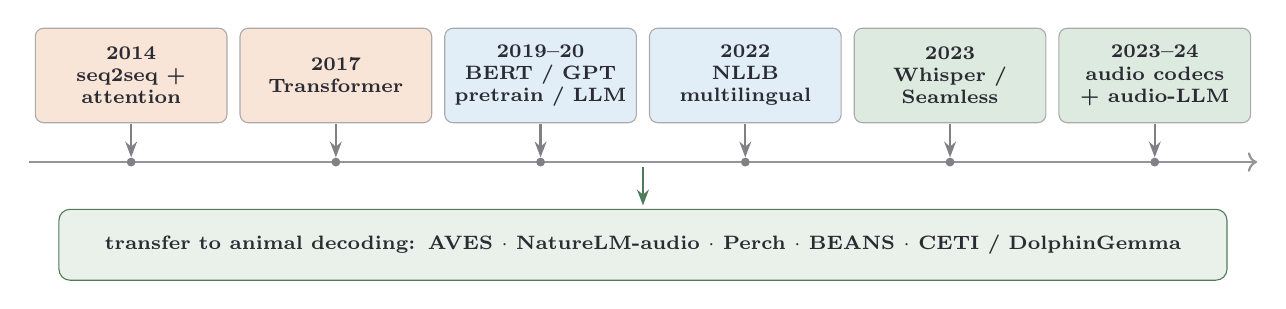
\begin{tikzpicture}[x=1cm,y=1cm,
  box/.style={rectangle, rounded corners=3pt, draw=ink!40, fill=#1, text=ink,
    align=center, text width=2.2cm, minimum height=1.2cm, font=\scriptsize\bfseries},
  arr/.style={-{Stealth[length=2mm]}, thick, ink!60}
]
% milestone boxes (year + mechanism)
\node[box=paw!30]  at (1.1,1.1)  {2014\\seq2seq +\\attention};
\node[box=paw!30]  at (3.7,1.1)  {2017\\Transformer};
\node[box=sky!30]  at (6.3,1.1)  {2019--20\\BERT / GPT\\pretrain / LLM};
\node[box=sky!30]  at (8.9,1.1)  {2022\\NLLB\\multilingual};
\node[box=sage!30] at (11.5,1.1) {2023\\Whisper /\\Seamless};
\node[box=sage!30] at (14.1,1.1) {2023--24\\audio codecs\\+ audio-LLM};
% timeline axis
\draw[->, thick, ink!50] (-0.2,0) -- (15.4,0);
\foreach \x in {1.1,3.7,6.3,8.9,11.5,14.1}{
  \fill[ink!60] (\x,0) circle (1.6pt);
  \draw[arr] (\x,0.48) -- (\x,0.06);
}
% transfer band
\draw[arr, sagedeep] (7.6,-0.06) -- (7.6,-0.55);
\node[rectangle, rounded corners=4pt, draw=sagedeep, fill=sage!20, text=ink,
  align=center, text width=14.6cm, minimum height=0.9cm, font=\scriptsize\bfseries]
  at (7.6,-1.05) {transfer to animal decoding: AVES $\cdot$ NatureLM-audio $\cdot$ Perch $\cdot$ BEANS $\cdot$ CETI / DolphinGemma};
\end{tikzpicture}
\caption{\textbf{The human translation / Transformer genealogy, condensed.}
Each layer supplies a tool that animal decoding inherits (acoustic encoding,
discretization, sequence modeling, multilingual transfer) or lacks (a
reference corpus, shared grounding). The lower band marks where the toolkit
has already been pointed at animals.}
\label{fig:genealogy}
\end{figure}

Statistical MT treated translation as noisy-channel decoding over phrase
tables learned from parallel corpora such as Europarl~\cite{koehn2004europarl}
and OPUS~\cite{tiedemann2012opus}, toolkitted by Moses~\cite{koehn2005moses}.
The neural turn replaced hand-built phrases with end-to-end encoder--decoder
learning~\cite{sutskever2014seq2seq,cho2014rnn}, and the decisive ingredient
was attention, a soft learned alignment between source and target
positions~\cite{bahdanau2015attention,luong2015effective}. Convolutional
variants competed briefly~\cite{gehring2017conv}, and production systems
showed that deep recurrent attention models could be deployed at
scale~\cite{wu2016gnmt,ott2018scaling}. Two data-side inventions proved as
important as the architecture: subword segmentation (BPE), which composes
rare words from frequent pieces~\cite{sennrich2016bpe}, and back-translation,
which manufactures parallel signal from monolingual
text~\cite{sennrich2016improving,edunov2018backtrans}. Both speak directly to
the animal case: BPE is a recipe for discretizing a continuous signal into
reusable units, back-translation a recipe for learning when no parallel
corpus exists.

The Transformer dispensed with recurrence entirely~\cite{vaswani2017attention},
and its real legacy is that it made pretraining scalable: masked language
modeling (BERT)~\cite{devlin2019bert}, causal modeling
(GPT)~\cite{radford2018gpt,radford2019gpt2,brown2020gpt3}, and seq2seq
denoising (T5, BART)~\cite{raffel2020t5,lewis2020bart} turned massive
unlabeled corpora into general-purpose representations, with refinements
(RoBERTa, XLNet, ELECTRA, DeBERTa) establishing that the objective and data
regime matter more than architectural
cleverness~\cite{liu2019roberta,yang2019xlnet,clark2020electra,he2021deberta}.
Contextual embeddings had already shown the value of pretraining over
static vectors (word2vec, GloVe, ELMo,
ULMFiT)~\cite{mikolov2013word2vec,pennington2014glove,peters2018elmo,howard2018ulmfit}.
Scaling laws make returns predictable~\cite{kaplan2020scaling},
compute-optimal training clarifies the data/scale
trade-off~\cite{hoffmann2022chinchilla}, and the foundation-model paradigm
frames both opportunity and risk~\cite{bommasani2021foundation}. For
bioacoustics the lesson is that a large unlabeled corpus of vocalizations,
pretrained with a masked or contrastive objective, is the right starting
point.

Human MT's most encouraging result for animal decoding is that quality does
not require a bespoke parallel corpus per language pair. Shared-encoder
multilingual models enable zero-shot
transfer~\cite{johnson2017multilingual,firat2016multiway}; cross-lingual
pretraining (XLM, XLM-R, mBART, multilingual BERT) shares structure across
languages~\cite{conneau2019xlm,conneau2020xlmr,liu2020mbart,pires2019mbert};
mined parallelism (WikiMatrix, CCAligned) plus many-to-many training (M2M-100,
NLLB) brought hundreds of low-resource languages into
scope~\cite{schwenk2021wikimatrix,elkishky2020ccaligned,fan2021beyond,costajussa2022nllb,nllb2024scaling};
and fully unsupervised MT is possible from monolingual corpora
alone~\cite{artetxe2018unsupervised,lample2018unsupervised}. This is the
closest human analogue to the animal situation: a target with no parallel
corpus, where structure must be bootstrapped from raw signal and transferred
from better-resourced relatives.

Translation then moved end-to-end to speech: listen-and-translate proofs of
concept~\cite{berard2016listen}, direct speech
translation~\cite{weiss2017speech}, direct speech-to-speech
models~\cite{jia2019direct}, and unified multilingual multimodal systems
(SeamlessM4T, Seamless)~\cite{seamless2023m4t,seamless2024streaming}. The
acoustic-encoder-plus-semantic-decoder template is exactly what a genuine
animal translator would need, and it is engineerable when the source is
human language. What animals lack is the evaluation layer: human MT rests on
accumulated reference translations, BLEU~\cite{papineni2002bleu},
METEOR~\cite{denkowski2014meteor}, and learned metrics such as
COMET~\cite{rei2020comet}, validated against expert
judgment~\cite{freitag2021experts} and adjudicated annually at
WMT~\cite{bojar2018wmt,barrault2019wmt,kocmi2022wmt}. Every one of these
presupposes a ground-truth target sentence.

Open and proprietary LLMs (LLaMA, Llama~2, GPT-4, Gemini, Claude,
Gemma)~\cite{touvron2023llama,touvron2023llama2,openai2023gpt4,gemini2024,anthropic2024claude,gemma2024},
instruction tuning~\cite{ouyang2022instruct}, and chain-of-thought
reasoning~\cite{wei2022chain} supply the semantic and interactive layer;
vision-language models (CLIP, Flamingo, LLaVA,
BLIP-2)~\cite{radford2021clip,alayrac2022flamingo,liu2023llava,li2023blip2}
show how to bind a non-linguistic modality to language, the exact operation
a dog translator attempts when grounding a bark to a context.

A bark is not human speech, so the acoustic front-end matters. The decisive
idea is to learn a general representation from raw unlabeled waveform and
fine-tune on small labeled tasks: CPC~\cite{vandenoord2018cpc},
wav2vec~\cite{schneider2019wav2vec}, wav2vec~2.0~\cite{baevski2020wav2vec2},
HuBERT~\cite{hsu2021hubert}, WavLM~\cite{chen2022wavlm}, and
data2vec~\cite{baevski2022data2vec,baevski2023data2vec2}. Two extensions
matter directly for animals: wav2vec-U learns recognition without any
transcriptions~\cite{baevski2021wav2vecu}, and multilingual scaling (XLS-R,
MMS, USM) pushes one encoder across thousands of
languages~\cite{babu2022xlsr,pratap2023mms,zhang2023usm}. The
transcription-free recipe is the closest human precedent for a target with
no parallel corpus.

Recognition architectures solve the alignment problem in two regimes: CTC
marginalizes over all alignments between frames and
labels~\cite{graves2006ctc,graves2013speech,amodei2016deepspeech2}, while
attention-based listen-attend-spell learns a soft
alignment~\cite{chan2016las}; the Conformer marries convolution to
self-attention~\cite{gulati2020conformer}. For animal signals the problem is
the same in form but harder in substance, because there is no canonical
label sequence to align to. None of this would exist without shared data
and evaluation: LibriSpeech~\cite{panayotov2015librispeech}, Common
Voice~\cite{ardila2020commonvoice}, Multilingual
LibriSpeech~\cite{pratap2020mls}, TIMIT and
Switchboard~\cite{garofolo1993timit,godfrey1992switchboard}, and benchmarks
such as SUPERB~\cite{yang2021superb} and
CoVoST~\cite{wang2020covost,wang2021covost2}. The absence of a ``LibriSpeech
of barks'' is a concrete, fixable bottleneck.

A second lineage turns waveform into discrete tokens a language model can
predict: WaveNet~\cite{vandenoord2016wavenet},
VQ-VAE~\cite{vandenoord2017vqvae}, Jukebox~\cite{dhariwal2020jukebox},
SoundStream and EnCodec~\cite{zeghidour2021soundstream,defossez2022encodec},
AudioLM~\cite{borsos2023audiolm} and its music and sound
successors~\cite{agostinelli2023musiclm,copet2023musicgen,kreuk2023audiogen},
VALL-E~\cite{wang2023valle}, UniAudio~\cite{yang2024uniaudio}, and audio-LLMs
(AudioPaLM, SALMONN, Qwen-Audio)~\cite{rubenstein2023audiopalm,tang2024salmonn,chu2024qwenaudio}.
This is the discretization step a ``bark alphabet'' would require, the
strategy Project CETI applied to whale codas~\cite{sharma2024whale}.

The same representation revolution in vision, AlexNet and
ImageNet~\cite{krizhevsky2012alexnet,deng2009imagenet,russakovsky2015imagenet},
ResNet~\cite{he2016resnet}, and the Vision
Transformer~\cite{dosovitskiy2021vit}, is the lineage DogFACS-style facial
analysis rides on (Section~\ref{sec:biology}). And the toolkit has been
pointed at animals: BirdNET~\cite{kahl2021birdnet}, the reviews charting
computational bioacoustics~\cite{stowell2022review,stowell2014automatic},
AVES~\cite{hagiwara2023aves}, NatureLM-audio~\cite{robinson2024naturelm},
Perch~\cite{ghani2023perch}, BEANS~\cite{hagiwara2023beans}, and
OpenBEATs~\cite{openbeats2025}. The transfer is measured, not assumed:
fine-tuned animal-audio encoders report gains over from-scratch baselines on
BEANS and BirdSet. What none supplies is a reference translation; they
classify, embed, and retrieve, but do not render a bark as a sentence with
measured fidelity. The engineering of the front-end is largely solved; the
missing piece is semantic, not acoustic.

\begin{table}[htbp]
\centering
\caption{The human translation / Transformer genealogy and its transfer
value to animal decoding. ``Transfer value'' is our assessment.}
\label{tab:genealogy}
\footnotesize
\setlength{\tabcolsep}{4pt}
\begin{tabular}{@{}p{0.8cm}p{3.4cm}p{3.4cm}p{5.6cm}@{}}
\toprule
\textbf{Year} & \textbf{Milestone} & \textbf{Key mechanism} & \textbf{Transfer value to animals} \\
\midrule
2006 & CTC~\cite{graves2006ctc} & alignment-free labeling & label variable-length vocalizations \\
2014 & seq2seq~\cite{sutskever2014seq2seq,cho2014rnn} & encoder--decoder & signal sequence $\to$ symbol sequence \\
2015 & attention~\cite{bahdanau2015attention} & soft alignment & align bark segments to labels \\
2016 & BPE / back-translation~\cite{sennrich2016bpe,sennrich2016improving} & subwords; synthetic parallelism & discretize; bootstrap without parallel data \\
2017 & Transformer~\cite{vaswani2017attention} & self-attention & the universal backbone \\
2017 & multilingual NMT~\cite{johnson2017multilingual} & shared encoder, zero-shot & one encoder across species \\
2019--20 & BERT / GPT / T5~\cite{devlin2019bert,brown2020gpt3,raffel2020t5} & masked / causal pretraining & foundation encoder from raw signal \\
2021 & ViT / CLIP~\cite{dosovitskiy2021vit,radford2021clip} & cross-modal transformers & bind non-linguistic modality to language \\
2022 & NLLB / Chinchilla~\cite{costajussa2022nllb,hoffmann2022chinchilla} & mined parallel; compute-optimal & low-resource recipe; data-vs-scale trade-off \\
2023 & LLMs / Whisper / Seamless~\cite{openai2023gpt4,radford2023whisper,seamless2023m4t} & scale; weak-supervision ASR & semantic layer; robust acoustic encoder \\
2024 & NLLB (Nature)~\cite{nllb2024scaling} & 200 languages deployed & proof that low-resource scale works \\
\bottomrule
\end{tabular}
\end{table}

\begin{table}[htbp]
\centering
\caption{The speech/audio foundation-model toolkit and its transfer value.
SSL = self-supervised; codec = discrete acoustic tokens.}
\label{tab:audio}
\footnotesize
\setlength{\tabcolsep}{4pt}
\begin{tabular}{@{}p{4.6cm}p{1.6cm}p{7.0cm}@{}}
\toprule
\textbf{Model / family} & \textbf{Type} & \textbf{Transfer value to animals} \\
\midrule
wav2vec~2.0 / HuBERT / data2vec~\cite{baevski2020wav2vec2,hsu2021hubert,baevski2022data2vec} & SSL & foundation bark encoder from unlabeled audio \\
wav2vec-U~\cite{baevski2021wav2vecu} & SSL & learn without a parallel corpus \\
XLS-R / MMS / USM~\cite{babu2022xlsr,pratap2023mms,zhang2023usm} & SSL & one encoder across species \\
CTC / LAS / Conformer~\cite{graves2006ctc,chan2016las,gulati2020conformer} & ASR & map variable-length signal to labels \\
Whisper~\cite{radford2023whisper} & ASR & robust off-the-shelf acoustic encoder \\
LibriSpeech / Common Voice / SUPERB~\cite{panayotov2015librispeech,ardila2020commonvoice,yang2021superb} & data & template for a ``bark corpus'' \\
SoundStream / EnCodec~\cite{zeghidour2021soundstream,defossez2022encodec} & codec & discretize vocalizations into tokens \\
AudioLM / VALL-E / UniAudio~\cite{borsos2023audiolm,wang2023valle,yang2024uniaudio} & codec-LM & search for sequence structure \\
AudioPaLM / SALMONN / Qwen-Audio~\cite{rubenstein2023audiopalm,tang2024salmonn,chu2024qwenaudio} & audio-LLM & bind acoustic signal to language \\
AVES / NatureLM / Perch / BEANS~\cite{hagiwara2023aves,robinson2024naturelm,ghani2023perch,hagiwara2023beans} & bioacoustic & cross-species transfer, already realized \\
\bottomrule
\end{tabular}
\end{table}

\section{Speech and Audio Foundation Models: The Acoustic Toolkit}
\label{sec:foundationaudio}

Section~\ref{sec:humanmt} traced the translation stack whose \emph{source} is
already human language. A bark is not. To turn a continuous, noisy,
variable-length vocalization into something a translator could consume, one
needs the acoustic front-end and the audio-token machinery that the speech
community built for itself. This section catalogs that toolkit from a
computer-science standpoint---self-supervised encoders, recognition
architectures, the corpora and benchmarks that made scale possible, neural
audio codecs, and audio--language models---and asks, for each, what an animal
decoder inherits. The recurring lesson is that \emph{the engineering of the
front-end is largely solved; the missing piece is semantic, not acoustic}.

\subsection{Self-supervised speech representation learning}
The decisive idea is to learn a general acoustic representation from raw,
unlabeled waveform, then fine-tune on a small labeled task. Contrastive
Predictive Coding (CPC) showed that predicting future latent frames yields
transferable features~\cite{vandenoord2018cpc}; wav2vec extended this with a
contrastive objective over a discrete vocabulary~\cite{schneider2019wav2vec};
and wav2vec~2.0 combined a convolutional feature encoder, a quantized latent
space, and a masked Transformer to reach strong recognition with only minutes
of transcribed audio~\cite{baevski2020wav2vec2}. HuBERT replaced the
contrastive target with masked prediction of offline-clustered
units~\cite{hsu2021hubert}, WavLM added denoising and speaker-aware
pretraining~\cite{chen2022wavlm}, and data2vec unified the masked-prediction
objective across speech, vision, and text~\cite{baevski2022data2vec}, with a
faster successor in data2vec~2~\cite{baevski2023data2vec2}. Two extensions
matter directly for animals: wav2vec-U learns to recognize speech
\emph{without any transcriptions} by adversarially aligning discrete units to
a language model~\cite{baevski2021wav2vecu}, and multilingual scaling
(XLS-R, MMS, USM) pushes a single encoder across dozens to thousands of
languages~\cite{babu2022xlsr,pratap2023mms,zhang2023usm}. The animal analogue
is exact: a large unlabeled corpus of barks, pretrained with a masked or
contrastive objective, is the correct starting point, and the
transcription-free recipe is the closest human precedent for a target with no
parallel corpus.

\subsection{Recognition architectures and the alignment problem}
Before Transformers, end-to-end recognition was built on recurrent networks
with two alignment regimes. Connectionist Temporal Classification (CTC)
marginalizes over all alignments between input frames and output
labels~\cite{graves2006ctc}, and deep recurrent CTC systems scaled to
end-to-end speech recognition~\cite{graves2013speech,amodei2016deepspeech2};
attention-based listen-attend-spell models instead learn a soft
alignment~\cite{chan2016las}. The Conformer married convolution with
self-attention to capture both local and global acoustic
structure~\cite{gulati2020conformer}. For animal signals the alignment
problem is the same in form---a variable-length vocalization must be mapped
to a variable-length label sequence---but harder in substance, because there
is no canonical label sequence to align to (Section~\ref{sec:eval}).

\subsection{Corpora and benchmarks that made scale possible}
None of the above would exist without shared data and evaluation. LibriSpeech
provided a thousand hours of read audiobook
speech~\cite{panayotov2015librispeech}; Common Voice crowdsourced a massively
multilingual corpus~\cite{ardila2020commonvoice}; Multilingual LibriSpeech
extended read speech across languages~\cite{pratap2020mls}; and the older
TIMIT and Switchboard corpora anchored phonetic and conversational
research~\cite{garofolo1993timit,godfrey1992switchboard}. Benchmarks then
standardized what ``good'' means: SUPERB probes a frozen representation across
many speech tasks~\cite{yang2021superb}, while CoVoST and CoVoST~2 supply
speech-translation references~\cite{wang2020covost,wang2021covost2}. The
bioacoustic community is only now building the equivalent infrastructure
(BEANS, BirdSet; Section~\ref{sec:crossspecies}), and the absence of a
``LibriSpeech of barks'' is a concrete, fixable bottleneck.

\subsection{Neural audio codecs and discrete acoustic tokens}
A second lineage turns waveform into \emph{discrete tokens} that a language
model can predict. WaveNet modeled raw audio autoregressively~\cite{vandenoord2016wavenet};
VQ-VAE introduced a learned discrete latent codebook~\cite{vandenoord2017vqvae};
Jukebox showed that hierarchical VQ-VAEs could generate coherent
music~\cite{dhariwal2020jukebox}. SoundStream and EnCodec made neural audio
compression practical with residual vector
quantization~\cite{zeghidour2021soundstream,defossez2022encodec}. AudioLM then
demonstrated that a language model over these tokens can generate long-range
coherent audio without any text~\cite{borsos2023audiolm}, and the recipe
generalized to music (MusicLM, MusicGen) and general sound
(AudioGen)~\cite{agostinelli2023musiclm,copet2023musicgen,kreuk2023audiogen}.
VALL-E treated text-to-speech as neural codec language
modeling~\cite{wang2023valle}; UniAudio pushed toward a single foundation model
for many audio tasks~\cite{yang2024uniaudio}; and AudioPaLM, SALMONN, and
Qwen-Audio fused speech/audio encoders with large language
models~\cite{rubenstein2023audiopalm,tang2024salmonn,chu2024qwenaudio}. This is
precisely the discretization step a ``bark alphabet'' would require: if
vocalizations can be compressed into reusable tokens, sequence models can
search for structure---the strategy Project CETI applied to whale
codas~\cite{sharma2024whale}.

\subsection{The visual backbone analogy}
The same representation-learning revolution happened in vision, and the
analogy clarifies what transfers. AlexNet's ImageNet win established deep
convolutional features as general-purpose~\cite{krizhevsky2012alexnet,deng2009imagenet,russakovsky2015imagenet};
residual networks made very deep models trainable~\cite{he2016resnet}; and the
Vision Transformer later showed the Transformer backbone works on pixels as
well as tokens~\cite{dosovitskiy2021vit}. DogFACS-style facial analysis
(Section~\ref{sec:biology}) rides directly on this lineage. The lesson is that
a modality becomes tractable once a large pretrained backbone exists---and
that the backbone, not the task head, is where the value lives.

\subsection{Bioacoustic foundation models}
Finally, the toolkit has been pointed at animals. BirdNET demonstrated
large-scale, consumer-grade bird identification from
audio~\cite{kahl2021birdnet}; comprehensive reviews chart both the promise and
the methodological pitfalls of computational
bioacoustics~\cite{stowell2022review,stowell2014automatic}. Self-supervised
AVES~\cite{hagiwara2023aves}, the audio--language NatureLM-audio
model~\cite{robinson2024naturelm}, Google's Perch embeddings~\cite{ghani2023perch},
the BEANS benchmark~\cite{hagiwara2023beans}, and open general-purpose audio
encoders such as OpenBEATs~\cite{openbeats2025} together show that the
human speech recipe---pretrain on raw audio, transfer to many tasks---works
across species. What none of them supplies is a \emph{reference translation}:
they classify, embed, and retrieve, but they do not, and cannot yet, render a
bark as a sentence with measured fidelity. Table~\ref{tab:audio} condenses the
toolkit and its transfer value.

\begin{table}[htbp]
\centering
\caption{The speech/audio foundation-model toolkit and its transfer value to
animal decoding. ``Transfer value'' is our assessment. SSL = self-supervised;
ASR = automatic speech recognition; codec = discrete acoustic tokens.}
\label{tab:audio}
\small
\setlength{\tabcolsep}{4pt}
\begin{tabular}{@{}p{3.0cm}p{1.8cm}p{3.4cm}p{5.1cm}@{}}
\toprule
\textbf{Model / family} & \textbf{Type} & \textbf{Objective / data} & \textbf{Transfer value to animals} \\
\midrule
CPC / wav2vec / wav2vec~2.0~\cite{vandenoord2018cpc,schneider2019wav2vec,baevski2020wav2vec2} & SSL & contrastive / masked, raw audio & foundation bark encoder from unlabeled audio \\
HuBERT / WavLM / data2vec~\cite{hsu2021hubert,chen2022wavlm,baevski2022data2vec,baevski2023data2vec2} & SSL & masked unit prediction & robust, denoised vocalization features \\
wav2vec-U~\cite{baevski2021wav2vecu} & SSL & transcription-free & learn without a parallel corpus \\
XLS-R / MMS / USM~\cite{babu2022xlsr,pratap2023mms,zhang2023usm} & SSL & 100s--1000s of languages & one encoder across species \\
CTC / LAS / Conformer~\cite{graves2006ctc,chan2016las,gulati2020conformer} & ASR & alignment-free / attention & map variable-length signal to labels \\
Whisper~\cite{radford2023whisper} & ASR & 680k h weak supervision & robust off-the-shelf acoustic encoder \\
LibriSpeech / Common Voice / SUPERB~\cite{panayotov2015librispeech,ardila2020commonvoice,yang2021superb} & data & corpora + benchmarks & template for a ``bark corpus'' \\
SoundStream / EnCodec~\cite{zeghidour2021soundstream,defossez2022encodec} & codec & residual VQ & discretize vocalizations into tokens \\
AudioLM / VALL-E / UniAudio~\cite{borsos2023audiolm,wang2023valle,yang2024uniaudio} & codec-LM & token language modeling & search for sequence structure \\
AudioPaLM / SALMONN / Qwen-Audio~\cite{rubenstein2023audiopalm,tang2024salmonn,chu2024qwenaudio} & audio-LLM & audio + text fusion & bind acoustic signal to language \\
AVES / NatureLM / Perch / BEANS~\cite{hagiwara2023aves,robinson2024naturelm,ghani2023perch,hagiwara2023beans} & bioacoustic & animal audio SSL & cross-species transfer, already realized \\
\bottomrule
\end{tabular}
\end{table}
\section{Transfer Feasibility: What Survives Contact with Animal Signals}
\label{sec:transfer}

We now have two stacks in view: the human translation genealogy
(Section~\ref{sec:humanmt}) and the speech/audio toolkit
(Section~\ref{sec:foundationaudio}). The decisive question is not whether these
tools are powerful---they are---but which of their \emph{presuppositions}
survive when the source is a dog rather than a human. This section audits the
transfer component by component, grounding the audit in the machine-learning
literature on transfer, representation, grounding, and compositionality. The
result, summarized in Table~\ref{tab:transfer}, is a clear pattern:
\emph{the acoustic and representational layers transfer almost intact; the
semantic and evaluative layers do not transfer at all.}

\subsection{Transfer learning: the formal picture}
Transfer learning formalizes when knowledge from a source domain helps in a
target domain~\cite{pan2010transfer,zhuang2021transfer}. Deep features are
often transferable, with generality decreasing as one moves from early to
late layers~\cite{yosinski2014transferable}. This is the optimistic half of
the story: an encoder pretrained on human speech or general audio can be
fine-tuned on barks, and cross-species bioacoustic models already demonstrate
the gain~\cite{hagiwara2023aves,ghani2023perch}. But transfer of
\emph{features} is not transfer of \emph{semantics}. The source domain of human
MT carries a target language with shared reference; the animal target domain
carries no such thing. Feature transfer succeeds precisely where the task is
classification; it cannot manufacture a reference translation that the source
domain never had.

\subsection{Representation-learning foundations}
The machinery that makes transfer possible is the standard deep-learning
stack: backpropagation~\cite{rumelhart1986backprop}, long short-term memory for
sequences~\cite{hochreiter1997lstm}, the deep-learning synthesis of
LeCun, Bengio, and Hinton~\cite{lecun2015deep,bengio2013representation,goodfellow2016deep},
and the optimization and regularization practices (Adam,
dropout) that make large models trainable~\cite{kingma2015adam,srivastava2014dropout}.
These are modality-agnostic: nothing in them assumes human language. A bark
encoder built from the same components is therefore engineerable, and indeed
AVES and NatureLM-audio are built from exactly
them~\cite{hagiwara2023aves,robinson2024naturelm}. The foundations transfer
without remainder; the bottleneck is downstream.

\subsection{The symbol-grounding problem}
Here the transfer breaks. Human translation is grounded: source and target
symbols alike refer to a shared world of objects, actions, and
states~\cite{harnad1990grounding}. A model trained only on text inherits this
grounding indirectly through human usage, but the limits of that inheritance
are well documented---text-only models lack the sensorimotor experience that
gives words their meaning~\cite{bisk2020experience}. For a dog there is no
shared symbolic world to ground into. The dog's signal is grounded in
\emph{its} affective and motivational states, not in a public lexicon; mapping
it to an English sentence is not translation between two grounded languages
but an act of interpretation across an unbridgeable referential gap. This is
the technical content of the ``semantic gap'' thesis, and it is why grounding,
not model scale, is the binding constraint.

\subsection{Compositionality, systematicity, and what probing reveals}
Human language is compositional: the meaning of a whole is a function of the
meanings of its parts and their combination. Whether neural models learn this
is contested~\cite{hupkes2020compositionality}, and diagnostic benchmarks
(SCAN, systematic-generalization tests) show that standard architectures
often fail to generalize compositionally even when they fit the training
distribution~\cite{lake2018scan,lake2023systematic}. Probing studies further
show that what a model ``knows'' is task- and probe-dependent, and that
BERT-style representations encode syntax without necessarily encoding
meaning~\cite{conneau2018cram,rogers2020bertology}. The implication for animals
is twofold. First, even if a bark sequence had compositional structure
(Section~\ref{sec:feasibility}), our models might not recover it. Second, the
absence of compositionality in the \emph{signal}---the likely case for
dogs---means there is no recursive structure for a sequence model to exploit,
so the very property that makes human MT work is missing at the source.

\subsection{Generative and interactive methods: the validation loop}
Two further ML lineages matter not for decoding but for \emph{validation}.
Generative models---GANs~\cite{goodfellow2014gan}, denoising diffusion
models~\cite{ho2020ddpm}, and latent diffusion~\cite{rombach2022ldm}---could
synthesize candidate vocalizations for playback experiments, closing the loop
between hypothesis and animal response. Reinforcement learning---from
DQN~\cite{mnih2015dqn} through PPO~\cite{schulman2017ppo} to the
self-play paradigm of AlphaGo~\cite{silver2016alphago}---supplies the framework
for an interactive agent that learns which inferred intents predict the dog's
behavior. These are the tools that could turn an unfalsifiable interpretation
into a measured, closed-loop system (Section~\ref{sec:eval}). They transfer
well; what they require is an error signal, which the field currently lacks.

We stress that Table~\ref{tab:transfer} is an \emph{analytical framework}, not
an experimental result. Where a row says ``transfers,'' the claim is backed
by measured cross-species fine-tuning gains on BEANS and
BirdSet~\cite{hagiwara2023beans,openbeats2025}; where it says ``fails,'' the
claim rests on the absence of any reference corpus or shared lexicon
(Sections~\ref{sec:eval} and~\ref{sec:lessons}). The framework's value is that
it localizes \emph{where} the bottleneck sits, so effort is not spent scaling
the layers that already transfer.

\begin{table}[htbp]
\centering
\caption{Transfer-feasibility audit: what each layer of the human translation
stack presupposes, and whether that presupposition holds for animal signals.
Verdicts are our assessment.}
\label{tab:transfer}
\small
\setlength{\tabcolsep}{4pt}
\begin{tabular}{@{}p{2.8cm}p{4.4cm}p{4.4cm}p{2.0cm}@{}}
\toprule
\textbf{Component} & \textbf{Human MT presupposes} & \textbf{Animal reality} & \textbf{Verdict} \\
\midrule
Acoustic encoder & raw waveform, any language & raw waveform, any species & transfers \\
Self-supervision & large unlabeled corpus & large unlabeled barks exist & transfers \\
Subword / codec units & discrete reusable units & units discoverable (cf.\ CETI) & partial \\
Sequence model & recursive, compositional source & likely non-compositional signal & limited \\
Parallel corpus & bilingual reference text & no reference exists & fails \\
Grounding & shared public lexicon & private affective states & fails \\
Evaluation metric & ground-truth target sentence & no intended message to score & fails \\
Closed-loop validation & observable error signal & buildable via playback / RL & buildable \\
\bottomrule
\end{tabular}
\end{table}
\section{Seven Lessons from Human Translation for Animal Decoding}
\label{sec:lessons}

The previous sections catalogued tools and audited their transfer. This
section distills the exchange into seven concrete lessons---what the history
of human machine translation, read as a computer-science narrative, teaches
anyone attempting to decode an animal. Each lesson pairs a human-MT finding
with a prescription for animal work. Table~\ref{tab:lessons} collects them.

\subsection{Lesson 1: Pretrain on unlabeled signal before anything else}
The single most robust finding of the last decade is that a large unlabeled
corpus, pretrained with a masked or contrastive objective, beats a clever
architecture trained from scratch~\cite{devlin2019bert,baevski2020wav2vec2,liu2019roberta}.
The animal prescription is immediate: invest first in a large, open,
unlabeled corpus of dog vocalizations and a self-supervised encoder, exactly
as AVES and NatureLM-audio have done for animals
generally~\cite{hagiwara2023aves,robinson2024naturelm}. Architecture is not the
bottleneck; data regime is.

\subsection{Lesson 2: Discretize before you translate}
BPE showed that composing rare words from frequent subword units unlocks
generalization~\cite{sennrich2016bpe}; neural codecs showed the same for
audio~\cite{zeghidour2021soundstream,defossez2022encodec}; and Project CETI's
``phonetic alphabet'' showed it for whales~\cite{sharma2024whale}. The
prescription: before claiming to translate, discover whether barks admit a
small set of reusable, recombinable units. If they do not, the signal is not
language-like and the translation framing should be dropped.

\subsection{Lesson 3: Bootstrap when no parallel corpus exists}
Human MT learned to manufacture its own supervision:
back-translation~\cite{sennrich2016improving,edunov2018backtrans} and fully
unsupervised translation~\cite{artetxe2018unsupervised,lample2018unsupervised}
removed the need for a bespoke parallel corpus. Animals have no parallel
corpus and never will. The prescription is to build a synthetic loop:
generate candidate vocalizations, play them back, and score the animal's
response---the generative-plus-reinforcement recipe of
Section~\ref{sec:transfer}. The error signal must come from the animal, not
from a human annotator's intuition.

\subsection{Lesson 4: Share structure across related systems}
Multilingual models showed that one encoder can serve hundreds of languages,
with low-resource pairs benefiting from high-resource
relatives~\cite{johnson2017multilingual,costajussa2022nllb,fan2021beyond}. The
prescription: train across species and across individuals, letting wolves,
coyotes, and many dogs inform a shared canid encoder, rather than fitting a
bespoke model per dog. Cross-species transfer is the animal analogue of
low-resource MT, and it is already paying off~\cite{ghani2023perch,babu2022xlsr}.

\subsection{Lesson 5: Evaluation precedes the claim}
Human MT earned its credibility through reference corpora and shared
tasks---BLEU, WMT, learned metrics validated against expert
judgment~\cite{papineni2002bleu,bojar2018wmt,rei2020comet,freitag2021experts}.
The animal field has no reference and therefore no comparable discipline. The
prescription is the demarcation of Section~\ref{sec:eval}: define the task,
disclose the protocol, and refuse the word ``translator'' until an independent
error signal exists. A field that cannot measure cannot improve.

\subsection{Lesson 6: Grounding is the wall, not scale}
Scaling laws make returns predictable~\cite{kaplan2020scaling,hoffmann2022chinchilla},
which tempts the inference that a big enough model will eventually translate a
bark. But the symbol-grounding problem is not a data deficit; it is a
referential mismatch~\cite{harnad1990grounding,bisk2020experience}. No amount
of compute creates a shared lexicon where none exists. The prescription:
spend effort on grounding and validation, not on parameter count, for the
upper rungs. Scale helps Rungs~1--3; it cannot fix a category error at
Rung~5.

\subsection{Lesson 7: Separate the interface from the measurement}
Modern systems render fluent sentences with a language
model~\cite{brown2020gpt3,ouyang2022instruct}, and fluency is easily mistaken
for fidelity---the hallucination and faithfulness literature documents exactly
this failure~\cite{ji2023hallucination,maynez2020faithfulness}. The
prescription: treat the rendered sentence as a user-interface layer, clearly
labeled as interpretation, and never let its fluency count as evidence. The
honest number lives upstream, at the classifier; the sentence is packaging.

\begin{table}[htbp]
\centering
\caption{Seven lessons from human machine translation, each paired with a
prescription for animal decoding.}
\label{tab:lessons}
\small
\setlength{\tabcolsep}{4pt}
\begin{tabular}{@{}p{0.6cm}p{4.7cm}p{8.0cm}@{}}
\toprule
\textbf{\#} & \textbf{Human-MT finding} & \textbf{Prescription for animals} \\
\midrule
1 & pretraining beats architecture~\cite{devlin2019bert,baevski2020wav2vec2} & build a large unlabeled bark corpus + SSL encoder first \\
2 & subwords / codecs unlock generalization~\cite{sennrich2016bpe,sharma2024whale} & discover reusable bark units before claiming translation \\
3 & unsupervised / back-translation~\cite{artetxe2018unsupervised,sennrich2016improving} & bootstrap supervision via playback + RL, not annotators \\
4 & multilingual sharing helps low-resource~\cite{costajussa2022nllb,johnson2017multilingual} & one shared canid encoder across species and individuals \\
5 & references + shared tasks = credibility~\cite{papineni2002bleu,bojar2018wmt} & no error signal, no ``translator''; disclose protocols \\
6 & scaling laws predict returns~\cite{kaplan2020scaling} & scale helps Rungs 1--3; grounding, not scale, blocks Rung 5 \\
7 & fluency $\neq$ fidelity~\cite{ji2023hallucination,maynez2020faithfulness} & label the sentence as interface; score the classifier \\
\bottomrule
\end{tabular}
\end{table}
\section{Feasibility: Alchemy, Flight, or Perpetual Motion}
\label{sec:feasibility}

The templates introduced in Section~\ref{sec:intro} can now be adjudicated
against evidence. The strongest argument that decoding animal signals is
flight rather than alchemy is that it has already been done, repeatedly, in
other species. Vervet monkeys produce predator-specific alarm calls that
elicit appropriate escape responses, and habituation--dishabituation
experiments show the calls function as referential
labels~\cite{seyfarth1980vervet,cheney1990monkeys}. Prairie dogs encode
predator type, size, and color~\cite{slobodchikoff2009prairie}, chicken alarm
calls carry graded referential content~\cite{evans1993alarm}, the honeybee
waggle dance communicates distance and direction~\cite{vonfrisch1967dance},
bottlenose dolphins use signature whistles as individual
labels~\cite{janik1998whistles,king2013labels}, and chimpanzees inform
conspecifics of danger in a goal-directed way~\cite{crockford2012inform}.
Japanese tits go further, combining calls into compositional
sequences~\cite{suzuki2016compositional}, and formal-semantics analyses find
context-dependent, rule-governed meaning in animal
calls~\cite{schlenker2016formal}. Referential and compositional signaling
exists in nature, so decoding it is an engineering problem, not a category
error. The open question is whether dogs sit in this referential class; the
canine evidence places them closer to the affective end.

The dog, meanwhile, is a willing and readable partner. Domestication
reshaped its social cognition for life with
humans~\cite{hare2002domestication,frantz2016genomic}: dogs follow human
pointing and gaze better than chimpanzees~\cite{soproni2001comprehension},
look back to humans at unsolvable tasks~\cite{miklosi2003lookback}, show
reward-system activation to praise in fMRI~\cite{berns2012fmri}, possess
voice-sensitive brain regions homologous to
humans'~\cite{andics2014voice}, and lateralize tail-wagging by emotional
valence~\cite{quaranta2007tail}. A few dogs learn hundreds of object
names~\cite{kaminski2004rico,pilley2011chaser}, and soundboard-trained dogs
produce non-random, non-imitative two-button combinations and respond to
human button presses above
chance~\cite{bastos2024plos,bastos2024scirep,bastos2023interact}. The dog is
not a black box: it perceives human communicative intent, signals its own
states readably, and in controlled settings exchanges referential tokens.
Affect-and-intent decoding has empirical ground to stand on; it is flight
with a runway already built.

The pessimistic half of the verdict concerns Rung~5. The comparative
evidence suggests that the recursive, generative syntax human translation
presupposes, the ``faculty of language in the narrow sense,'' may be
uniquely human~\cite{hauser2002faculty,chomsky1957syntactic,hauser1996evolution}.
On this view the language instinct is a species-typical
adaptation~\cite{pinker1994instinct} rooted in shared
intentionality~\cite{tomasello2008origins}, and the cultural-evolution
literature shows how iterated learning and cumulative culture shape
linguistic structure into something no individual animal
invents~\cite{kirby2008cumulative,smith2003iterated}; even the statistical
universals of human language are signatures of a generative
system~\cite{zipf1949human}. If a dog's repertoire lacks this structure,
``translating its sentences'' is alchemy-like: not hard engineering but a
target that may not exist. The modality matters: this is not a
perpetual-motion proof. No conservation law forbids richer animal
signaling, and the compositionality results above keep the empirical
question open. Rung~5 is possibly ill-posed, not provably impossible.

The layered verdict, then: Rungs~1--2 are achieved flight; Rung~3 is flight
with a foothold; Rung~4 is flight in some species and an open question for
dogs; Rung~5 is alchemy-like. Nothing here is perpetual motion, and the
existence proofs guarantee that something real is achievable. The practical
consequence is to pour effort into the grounded, falsifiable lower rungs and
treat the upper rung as a hypothesis about the animal rather than a product
roadmap (Table~\ref{tab:proofs}).

\begin{table}[htbp]
\centering
\caption{Existence proofs and the feasibility template each supports.
Nothing here is ``perpetual motion'' (provably impossible).}
\label{tab:proofs}
\footnotesize
\setlength{\tabcolsep}{4pt}
\begin{tabular}{@{}p{3.4cm}p{8.0cm}p{2.2cm}@{}}
\toprule
\textbf{Claim} & \textbf{Existence proof} & \textbf{Template} \\
\midrule
Affect decodable (R2) & humans classify barks/growls~\cite{pongracz2005barks,farago2017growls}; tail lateralization~\cite{quaranta2007tail}; voice regions~\cite{andics2014voice} & flight (achieved) \\
Intent inferable (R3) & pointing~\cite{soproni2001comprehension}; look-back~\cite{miklosi2003lookback}; soundboard combos~\cite{bastos2024scirep} & flight (foothold) \\
Reference in animals (R4) & vervet \& prairie alarms~\cite{seyfarth1980vervet,slobodchikoff2009prairie}; dolphin labels~\cite{janik1998whistles}; bee dance~\cite{vonfrisch1967dance} & flight (species-dependent) \\
Compositionality (R4) & tit compositional calls~\cite{suzuki2016compositional}; formal semantics~\cite{schlenker2016formal} & flight (rare) \\
Dogs read human speech & fMRI reward~\cite{berns2012fmri}; word learning~\cite{kaminski2004rico,pilley2011chaser} & flight (achieved) \\
Open translation (R5) & no recursive syntax in dogs; narrow faculty possibly unique~\cite{hauser2002faculty,chomsky1957syntactic} & alchemy-like \\
Provably impossible? & no conservation law forbids signaling & not perpetual motion \\
\bottomrule
\end{tabular}
\end{table}

\section{What Dogs Actually Signal: The Biological Substrate}
\label{sec:biology}

Before asking whether a machine can translate a dog, we must ask what there
is to translate. Canine communication is multimodal, graded, and heavily
context-dependent. It is also, crucially, \emph{asymmetric}: much of what a
dog ``says'' is addressed to humans, and the dog's receptive understanding of
human signals far exceeds its productive repertoire. This section reviews
the channels and the evidence that each carries decodable information.
Table~\ref{tab:channels} summarizes the landscape.

\subsection{Vocalizations: barks, growls, whines}
The domestic dog is unusually vocal for a canid, a trait widely interpreted
as a product of domestication and paedomorphosis. The ELTE Budapest
ethology group has built the most systematic body of evidence on what barks
encode. Pongr\'acz and colleagues showed that human listeners can classify
barks recorded in different behavioral situations above
chance~\cite{pongracz2005barks}, and that acoustic parameters---fundamental
frequency, tonality, and inter-bark interval---carry emotional information
that listeners reliably extract~\cite{pongracz2006acoustic}. Later work
established that barks also carry \emph{individual identity}: listeners can
discriminate dogs from bark acoustics alone~\cite{molnar2006discriminate},
and machine classifiers applied to thousands of barks from a kennel of
Hungarian sheepdogs recovered both context and individual at rates well
above chance, with ``stranger at the fence'' and ``fight'' contexts most
separable and ``play'' least. Growls are even more informative: Farag\'o et
al.\ demonstrated that human listeners judge a dog's size and aggressive
intent from growl formants, and that growls produced in food-guarding versus
play contexts are acoustically and perceptually
distinct~\cite{farago2017growls}. Whines and whimpers, associated with
separation and submission, complete a repertoire that is graded rather than
discrete.

The engineering literature has begun to automate exactly these judgments.
The ICASSP 2018 study ``What is my dog trying to tell me?'' framed bark
analysis as automatic recognition of \emph{context} and \emph{perceived
emotion}~\cite{icassp2018dogbark}, explicitly building on the ELTE
psychophysics. The important nuance---which we will return to in
Section~\ref{sec:eval}---is that the target label is the \emph{human-perceived}
emotion or the \emph{eliciting context}, not the dog's ``intended message.''
The model learns a mapping that humans already agree on; it does not recover
a hidden sentence.

\subsection{The face: DogFACS and the ``puppy dog eyes'' effect}
Canine facial behavior is codable with the same rigor as human facial
action coding. DogFACS, the Dog Facial Action Coding
System~\cite{waller2013dogfacs}, adapts Ekman and Friesen's FACS to the
musculature of the dog face, defining action units (e.g., AU101, the inner
brow raiser) and ear action descriptors. Using DogFACS, Kaminski et al.\
showed that dogs produce markedly more facial movement---especially the
inner brow raiser that enlarges the apparent eye---when a human is
\emph{attending} to them than when the human's back is turned, and that the
presence of food does not drive the effect~\cite{kaminski2017attention}.
This is a striking result: it suggests the ``puppy dog eyes'' expression is
a \emph{communicative} signal tuned to human attention, possibly shaped by
selection during domestication, rather than a mere reflex of internal
state. A 2024 comparative study further reported that domestication
\emph{constrains} the dog's facial expressiveness relative to
wolves~\cite{sci2024domestication}, complicating any simple ``dogs emote
freely'' narrative.

Automated facial analysis is now an active computer-vision subfield.
Explainable CNN pipelines recognize emotional states from canine facial
action patterns~\cite{sci2022explainable}, improved optimization schemes
push expression-recognition accuracy~\cite{sci2023cnnewoa}, and 2025 work
automates emotional-expression analysis end to end~\cite{sci2025automated}
and standardizes facial landmark detection~\cite{sci2025landmarks}. These
are genuine advances---but, again, their labels are human-coded affective
categories or DogFACS action units, not propositions.

\subsection{The body: posture, tail, and gaze}
A large fraction of everyday canine signaling is postural: ear position,
tail carriage and wag direction, weight distribution, piloerection, and
gaze. Classic work reported lateralized tail-wagging biases tied to
approach versus withdrawal motivation, and the broader ethogram of
dominance, submission, play (the play bow), and stress is well documented in
the clinical literature. Body signals are often \emph{more} diagnostic than
vocalizations, a point commercial vendors themselves concede: Traini's
founder has stated that audio alone is insufficient and that combining body
language and facial expression raises accuracy. This is an implicit
admission that the ``translation'' is really multimodal affect
classification. Olfactory signaling---urine marking, pheromonal
communication---is enormously important to dogs but essentially inaccessible
to current consumer sensors, and we flag it as a blind spot rather than a
solved channel.

\subsection{Reception: dogs understand more than they say}
Any honest account must separate what dogs \emph{produce} from what they
\emph{comprehend}. The receptive side is impressive. Rico, a border collie,
provided the first evidence of ``fast mapping''---inferring a novel word's
referent by exclusion---in \emph{Science}~\cite{kaminski2004rico}. Chaser,
another border collie, was documented retrieving 1{,}022 named objects and
responding to simple noun--verb combinations~\cite{pilley2011chaser}. These
are exceptional, intensively trained individuals, but they establish an
upper bound on referential comprehension that is far higher than the
productive repertoire. The asymmetry matters: a future ``dialogue'' system
may succeed by letting dogs \emph{receive} structured human input (as
soundboards do) long before it can \emph{read} structured canine output.

\subsection{Soundboards: the closest thing to canine ``speech''}
The most direct attempt to give dogs a productive symbolic channel is the
augmentative interspecies communication (AIC) soundboard: a grid of buttons
that each speak a recorded word when pressed. Popularized by speech
pathologist Christina Hunger and the Instagram dog Bunny, the phenomenon is
now under controlled study by Federico Rossano's UC San Diego
\emph{TheyCanTalk} project, which tracks thousands of button-using pets
across dozens of countries. Two 2024 peer-reviewed papers anchor the
science. Bastos et al.\ (\emph{PLoS ONE}) showed that soundboard-trained dogs
respond appropriately to words such as ``play'' and ``outside'' whether the
word is spoken by the owner or triggered by an unfamiliar button-presser,
indicating word comprehension rather than cue-reading~\cite{bastos2024plos}.
A companion \emph{Scientific Reports} paper analyzed two-button
combinations and found them to be non-accidental, non-random, and
non-imitative---evidence of intentional, if linear,
combination~\cite{bastos2024scirep}. A 2025 review synthesizes the evidence
and the skepticism~\cite{animalcog2025review}. The consensus interpretation
is careful: the combinations look like associative sequences (name\,+\,action,
place\,+\,go), not recursive grammar; spatial and immediate concepts
(``outside,'' ``paw'') are robust, while temporal abstractions
(``yesterday,'' ``tomorrow'') are rare and inconsistent. Soundboards thus
demonstrate \emph{referential intent} on the third rung of our ladder---but
they do so by giving the dog a human-designed symbol set, not by decoding
the dog's natural signal.

\begin{table}[htbp]
\centering
\caption{Canine communication channels, the information they carry, and the
strongest evidence. ``Decodable today'' refers to validated, above-chance
machine or human inference on a defined label---not to sentence-level
translation.}
\label{tab:channels}
\small
\begin{tabular}{@{}p{2.5cm}p{4.1cm}p{4.0cm}p{2.6cm}@{}}
\toprule
\textbf{Channel} & \textbf{Information encoded} & \textbf{Key evidence} & \textbf{Decodable today} \\
\midrule
Bark & Affect, arousal, context, individual identity &
Pongr\'acz et al.~\cite{pongracz2005barks,pongracz2006acoustic};
Moln\'ar et al.~\cite{molnar2006discriminate} & Affect/context (above chance) \\
Growl & Body size, aggressive intent, resource-guarding vs.\ play &
Farag\'o et al.~\cite{farago2017growls} & Size/intent (human + ML) \\
Whine/whimper & Separation distress, submission & Ethological observation &
Coarse affect \\
Face (DogFACS) & Attention-directed signals, affective state &
Waller et al.~\cite{waller2013dogfacs}; Kaminski et al.~\cite{kaminski2017attention} &
Action units; affect (CNN) \\
Body/tail/gaze & Motivation, stress, play, social intent &
Clinical ethograms; wag-laterality studies & Posture classes \\
Olfaction & Identity, reproductive state, territory &
Scent-marking literature & \emph{Not} sensor-accessible \\
Reception (input) & Human word referents (up to 1{,}022) &
Kaminski et al.~\cite{kaminski2004rico}; Pilley \& Reid~\cite{pilley2011chaser} &
Comprehension, not production \\
Soundboard (AIC) & Referential intent via human symbols &
Bastos et al.~\cite{bastos2024plos,bastos2024scirep} &
Word-level intent (trained) \\
\bottomrule
\end{tabular}
\end{table}

\subsection{The takeaway}
The biological substrate is real and rich: dogs signal affect, arousal,
identity, motivation, and---with human scaffolding---referential intent.
What the substrate does \emph{not} contain is an open-ended generative
grammar. This single fact, more than any limitation of current models,
bounds what ``translation'' can mean. We formalize that bound next.
\section{The Translation Ladder}
\label{sec:ladder}

The phrase ``translate what a dog says'' smuggles in an assumption: that a
sentence-shaped meaning waits in the signal, the way a French sentence waits
behind its English translation. The biological record gives reason to doubt
this. We therefore replace the single verb with a ladder of five distinct
capabilities, each with its own input--output contract, its own notion of
ground truth, and its own distance from the present
(Figure~\ref{fig:ladder}).

\begin{figure}[t]
\centering
\resizebox{\textwidth}{!}{% Figure 1 — The Translation Ladder (hero figure).
% Compiled standalone via fig1_standalone.tex; also \input by sections/03_ladder.tex.
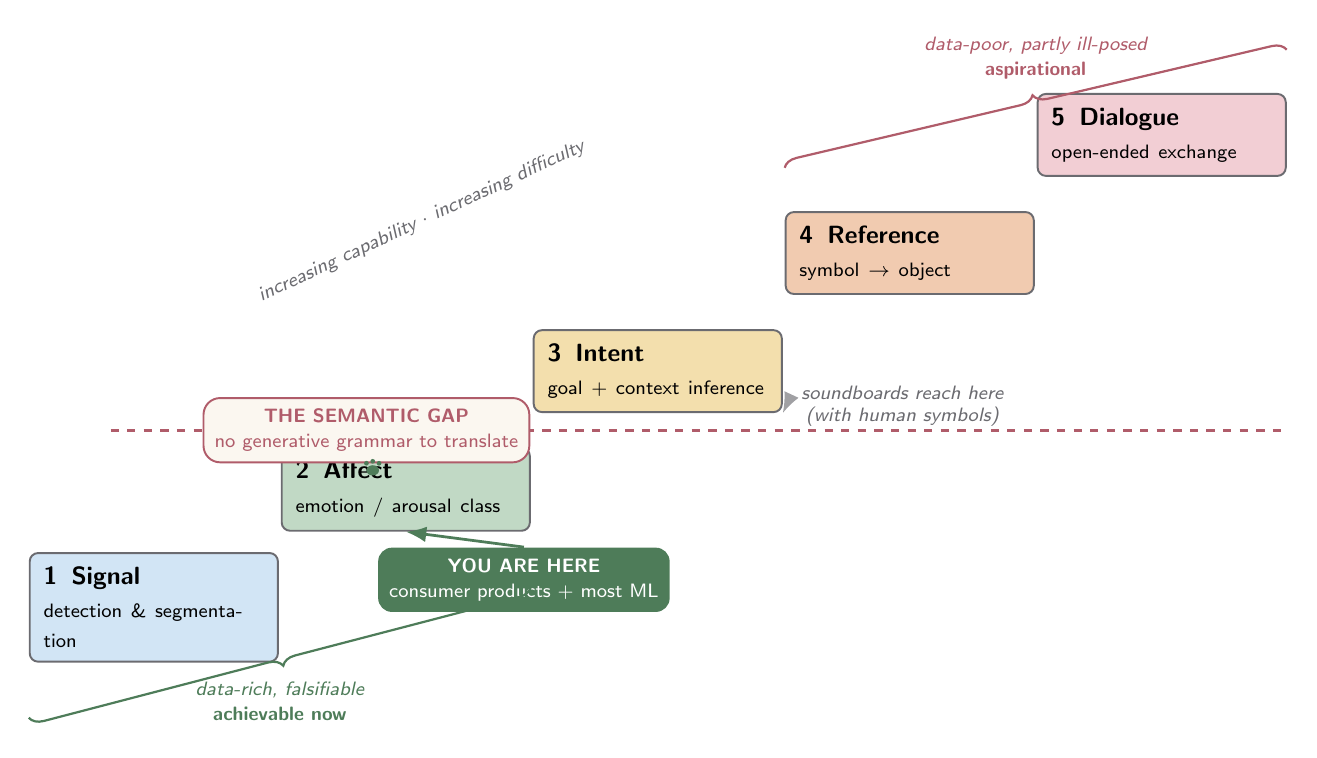
\begin{tikzpicture}[
  font=\sffamily,
  >={Latex[length=2.6mm,width=2mm]},
  block/.style={rounded corners=3pt,draw=ink!70,line width=0.7pt,
    minimum height=0.9cm,align=left,inner sep=5pt,text width=2.8cm,
    font=\sffamily\small},
  num/.style={font=\sffamily\bfseries\large},
  note/.style={font=\sffamily\scriptsize\itshape,text=ink!70},
  pill/.style={rounded corners=6pt,fill=cream,draw=rosedeep,line width=0.7pt,
    inner sep=4pt,font=\sffamily\scriptsize\bfseries,text=rosedeep,align=center},
]
  \node[block,fill=sky!45] (r1) at (0,0)
    {\num{1}\;\;\textbf{Signal}\\[1pt]\scriptsize detection \& segmentation};
  \node[block,fill=sage!55] (r2) at (3.2,1.5)
    {\num{2}\;\;\textbf{Affect}\\[1pt]\scriptsize emotion / arousal class};
  \node[block,fill=gold!55] (r3) at (6.4,3.0)
    {\num{3}\;\;\textbf{Intent}\\[1pt]\scriptsize goal + context inference};
  \node[block,fill=paw!60] (r4) at (9.6,4.5)
    {\num{4}\;\;\textbf{Reference}\\[1pt]\scriptsize symbol $\rightarrow$ object};
  \node[block,fill=rose!55] (r5) at (12.8,6.0)
    {\num{5}\;\;\textbf{Dialogue}\\[1pt]\scriptsize open-ended exchange};

  \node[note,rotate=25] at (3.4,4.9) {increasing capability $\cdot$ increasing difficulty};

  \draw[dashed,rosedeep,line width=1pt] (-0.55,2.25) -- (14.4,2.25);
  \node[pill] at (2.7,2.25)
    {THE SEMANTIC GAP\\[1pt]\mdseries no generative grammar to translate};

  \node[rounded corners=5pt,fill=sagedeep,text=white,inner sep=4pt,
    font=\sffamily\scriptsize\bfseries,align=center] (here) at (4.7,0.35)
    {YOU ARE HERE\\[1pt]\mdseries consumer products + most ML};
  \draw[->,sagedeep,line width=1pt] (here.north) -- (r2.south);
  \begin{scope}[shift={(2.78,1.74)},scale=0.5]
    \fill[sagedeep] (0,0) ellipse (0.16 and 0.13);
    \fill[sagedeep] (-0.16,0.18) circle (0.06);
    \fill[sagedeep] (0,0.23) circle (0.06);
    \fill[sagedeep] (0.16,0.18) circle (0.06);
  \end{scope}

  \node[note,align=center,anchor=west] at (8.1,2.55)
    {soundboards reach here\\(with human symbols)};
  \draw[->,ink!45,line width=0.7pt] (8.05,2.6) -- (r3.south east);

  \draw[decorate,decoration={brace,amplitude=5pt,mirror},sagedeep,line width=0.8pt]
    ($(r1.south west)+(0,-0.7)$) -- ($(r2.south east)+(0,-0.7)$)
    node[midway,below=7pt,note,text=sagedeep,align=center]
      {data-rich, falsifiable\\[1pt]\bfseries achievable now};
  \draw[decorate,decoration={brace,amplitude=5pt},rosedeep,line width=0.8pt]
    ($(r4.north west)+(0,0.55)$) -- ($(r5.north east)+(0,0.55)$)
    node[midway,above=7pt,note,text=rosedeep,align=center]
      {data-poor, partly ill-posed\\[1pt]\bfseries aspirational};
\end{tikzpicture}}
\caption{\textbf{The translation ladder.} Current consumer products and most
machine-learning work occupy \rung{Rung 2} (affect classification);
controlled soundboard studies reach \rung{Rung 3} (referential intent) but
only by supplying a human-designed symbol set. The dashed boundary marks the
\emph{semantic gap}: above it, the dog's natural signal lacks the recursive,
generative syntax that sentence-level translation presupposes, so the target
becomes possibly ill-posed rather than merely hard.}
\label{fig:ladder}
\end{figure}

\textbf{Rung 1, signal detection and segmentation}, asks only whether there
is a vocalization, where it begins and ends, and who produced it. This is a
classical detection problem with objective ground truth, and it is
essentially solved: bioacoustic detectors segment and attribute calls
reliably~\cite{ghani2023perch,hagiwara2023aves}, and individual
identification from bark acoustics is above
chance~\cite{molnar2006discriminate}. Nothing about Rung 1 requires
understanding.

\textbf{Rung 2, affect and arousal classification}, maps a signal to a small
set of affective categories or to continuous arousal/valence dimensions.
This is where nearly all commercial ``translators'' live and where the
peer-reviewed ML literature is strongest, because the labels are
human-perceived emotions or eliciting contexts that annotators can agree
on~\cite{pongracz2006acoustic,icassp2018dogbark,sci2022explainable}. Rung 2
is falsifiable and genuinely useful for welfare monitoring. Its limit is
that an emotion label is not a sentence; rendering ``fearful'' as ``I am
scared of the vacuum'' adds narrative the signal never contained.

\textbf{Rung 3, intent and context inference}, asks what the dog is trying
to do, given the surrounding context, and requires multimodal fusion and a
model of the dog's goals. Soundboard studies provide the cleanest evidence,
because the button press makes the intent explicit and
checkable~\cite{bastos2024plos,bastos2024scirep}, but the symbol set is
human-designed and trained. Rung 3 on natural signals is far less developed
and much harder to validate.

\textbf{Rung 4, referential semantics}, would map a spontaneous canine
signal to a specific referent without human-supplied symbols. Receptive
studies show dogs can understand such
mappings~\cite{kaminski2004rico,pilley2011chaser}, but a productive, open
referential vocabulary in natural dog communication has not been
demonstrated. This is the first rung where the translation framing strains:
there may be no stable symbol-to-referent dictionary to recover.

\textbf{Rung 5, open-ended dialogue}, is the folkloric dream: free,
generative, two-way conversation. It presupposes a recursive generative
grammar on the canine side, and the evidence of graded affective signals,
linear associative combinations, and no demonstrated syntax gives no
support for that presupposition. Rung 5 is therefore not merely distant; in
its strong form it is possibly ill-posed. A weaker engineered version,
structured human-to-dog input via soundboards with the dog responding
through trained symbols, is conceivable and already nascent.

The ladder converts a vague question into answerable ones: which rung, with
what ground truth, at what validated accuracy? It also explains the rhetoric
of the market, where vendors demonstrate Rung 2 while marketing Rung 5. The
rest of the survey uses it as a ruler.

\section{The Technical Pipeline: From Waveform to (Something Like) Meaning}
\label{sec:pipeline}

If genuine translation were possible, what would the system look like?
Drawing on the cross-species decoding literature, we decompose the problem
into four stages---\emph{encoding}, \emph{structure discovery},
\emph{semantic grounding}, and \emph{interactive validation}---and assess
the maturity of each for the canine case. The stages are not a waterfall so
much as a loop: validation feeds back into grounding, which constrains
structure, which shapes the encoder.

\subsection{Stage 1: self-supervised acoustic encoding}
The modern starting point is a self-supervised representation trained on
large, unlabeled audio. AVES (Animal Vocalization Encoder based on
Self-Supervision) adapts the HuBERT/wav2vec paradigm to animal sound and
shows that representations learned without labels transfer to downstream
bioacoustic tasks~\cite{hagiwara2023aves}. NatureLM-audio extends this to an
\emph{audio--language} foundation model: trained on text--audio pairs
spanning bioacoustics, speech, and music, it can detect vocalizations,
classify rare species, and even caption or generate animal sounds from
natural-language prompts, demonstrating transfer from speech and music to
bioacoustics~\cite{robinson2024naturelm}. Google DeepMind's Perch line and
the global birdsong embeddings show that a single encoder can serve many
taxa~\cite{ghani2023perch}. Standardized benchmarks---BEANS (the Benchmark
of Animal Sounds) and BirdSet---give these encoders a common evaluation
surface~\cite{hagiwara2023beans}, while open general-purpose encoders such
as OpenBEATs push state of the art on a majority of BEANS
subtasks~\cite{openbeats2025}. For dogs, the implication is that a strong
\emph{Rung 1--2} encoder is available off the shelf; the bottleneck is not
representation quality but labels and semantics.

\subsection{Stage 2: sequence-structure discovery}
Given an encoder, the next question is whether the signal has
\emph{combinatorial structure}---discrete units that recombine, the way
phonemes form words. This is where the flagship projects have produced
their most cited results. Project CETI's analysis of 8{,}719 sperm-whale
codas revealed a ``phonetic alphabet'': rhythm, tempo, rubato, and
ornamentation combine contextually, expanding the repertoire of
distinguishable forms by nearly an order of magnitude~\cite{sharma2024whale}.
Crucially, the authors are explicit that this describes \emph{form}, not
\emph{meaning}: the paper answers what the units are and how they combine,
not what most of them say. Google's DolphinGemma takes the language-model
route directly---a roughly 400-million-parameter Gemma-based model with a
SoundStream tokenizer, trained on the Wild Dolphin Project's four-decade
Atlantic spotted dolphin corpus, that predicts the next sound in a sequence
exactly as an LLM predicts the next token~\cite{google2025dolphingemma}.
CETI's WhAM (2025) similarly learns to complete masked clicks and to render
whale-like codas from other audio. The Earth Species Project's 2026
zebra-finch model (ZF-AIM) goes further, detecting, predicting, and
\emph{generating} calls in real time and engaging birds in turn-taking
exchanges.

The lesson for dogs is double-edged. On one hand, the methods are
species-agnostic and could be applied to bark sequences. On the other, the
structure these models find is \emph{statistical}, and predicting the next
sound is not understanding it. Yossi Yovel and others have warned that such
models may cluster calls by acoustic similarity while missing meaning
entirely---grouping signals that sound alike but signify different
things. For a repertoire as graded and context-bound as the dog's, the
prior probability of finding a clean combinatorial alphabet is lower than
for whale codas or birdsong.

\subsection{Stage 3: semantic grounding}
Structure without semantics is syntax without a dictionary. Grounding ties
a signal to the world: to the eliciting context, the dog's subsequent
behavior, the objects in view, the social partner. This is the hardest
stage and the one where dogs are paradoxically \emph{advantaged}, because
they live in richly instrumented human homes and their behavior is legible
to us. The soundboard paradigm is effectively a grounding
device~\cite{bastos2024plos,bastos2024scirep}: the button press, the spoken
word, and the consequent action (door opens, toy appears) form a
triangulated, checkable mapping. The Wild Dolphin Project's CHAT system
does the analogous thing underwater, pairing a synthetic whistle with a
coveted object (sargassum, a scarf) so that the dolphin can request it by
name~\cite{google2025dolphingemma}. The general principle---\emph{ground
symbols through interaction and consequence}, not through passive
correlation---is the field's most important methodological insight, and it
is exactly what consumer bark-to-sentence apps lack.

\subsection{Stage 4: interactive validation (playback)}
The final stage closes the loop: does the animal treat the model's output
as meaningful? The gold standard is the \emph{playback experiment}---play a
recorded or synthesized signal and observe whether the receiver responds
appropriately. Comparative ethology has used playbacks for decades to
establish that, e.g., vervet alarm calls refer to specific predators. The
Earth Species Project's interactive finch work and the CHAT dolphin
protocol are modern, model-driven versions. For dogs, a validation loop
would look like: infer an intent, emit a candidate signal or action, and
test whether the dog's behavior confirms the inference---with the
experimenter blind to the model's guess to avoid Clever-Hans contamination.
No consumer product does this; it is the dividing line between science and
entertainment.

\subsection{Maturity summary}
Table~\ref{tab:pipeline} rates each stage for the canine case. The pattern
is clear: the \emph{front} of the pipeline (encoding, structure) is
borrowable from the broader bioacoustics boom and is relatively mature; the
\emph{back} (grounding, validation) is where canine-specific, falsifiable
work is needed and where almost none of the commercial effort is directed.
This asymmetry---strong models, weak semantics, absent validation---is the
technical signature of the whole field.

\begin{table}[htbp]
\centering
\caption{Maturity of the four decoding stages for the canine case.
``Borrowable'' means general bioacoustic methods transfer directly;
``canine-specific'' means dedicated dog data and protocols are required.}
\label{tab:pipeline}
\small
\begin{tabular}{@{}p{2.7cm}p{4.6cm}p{2.5cm}p{3.0cm}@{}}
\toprule
\textbf{Stage} & \textbf{Representative method} & \textbf{Maturity} & \textbf{Canine status} \\
\midrule
Encoding & AVES, NatureLM-audio, Perch~\cite{hagiwara2023aves,robinson2024naturelm,ghani2023perch} &
High & Borrowable; Rung 1--2 ready \\
Structure & CETI alphabet, DolphinGemma, WhAM~\cite{sharma2024whale,google2025dolphingemma} &
Medium & Statistical only; meaning open \\
Grounding & Soundboards, CHAT object-labeling~\cite{bastos2024plos,google2025dolphingemma} &
Low--medium & Needs interaction data \\
Validation & Playback / closed-loop response & Low & Absent in products \\
\bottomrule
\end{tabular}
\end{table}
\section{Lessons from Other Species: Whales, Dolphins, and Finches}
\label{sec:crossspecies}

Dogs are not the first species for which decoding has been attempted, and
the comparison is instructive. The flagship projects differ from the canine
case in one decisive respect: their subjects often possess \emph{discrete,
culturally transmitted vocal units} (whale codas, dolphin signature
whistles, birdsong syllables) that invite combinatorial analysis. Dogs, by
contrast, signal with graded, context-bound affective displays. Reading the
cross-species literature through the ladder of Section~\ref{sec:ladder}
clarifies both what is transferable and what is not.
Figure~\ref{fig:roadmap} places these milestones on a capability timeline;
Table~\ref{tab:milestones} gives the details.

% ===========================================================================
% FIGURE 2 — Capability Roadmap (hero figure)
% ===========================================================================
\begin{figure}[t]
\centering
% Figure 2 — Capability Roadmap (hero figure).
% Compiled standalone via fig2_standalone.tex; also \input by sections/05_crossspecies.tex.
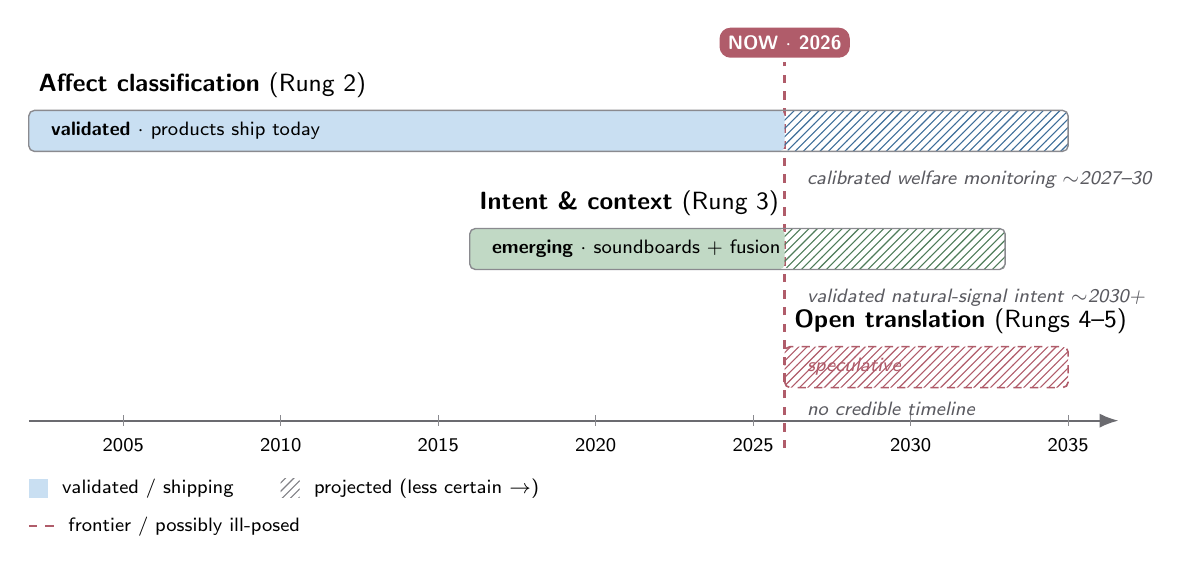
\begin{tikzpicture}[
  font=\sffamily,
  >={Latex[length=2.4mm,width=1.8mm]},
  x=0.40cm,y=1cm,
  tracktitle/.style={font=\sffamily\small\bfseries,anchor=south west},
  projection/.style={font=\sffamily\scriptsize\itshape,anchor=north west,text=ink!78},
  legend/.style={font=\sffamily\scriptsize,anchor=west},
]
  \draw[->,ink!70,line width=0.8pt] (0,0) -- (34.6,0);
  \foreach \yr/\x in {2005/3,2010/8,2015/13,2020/18,2025/23,2030/28,2035/33}{
    \draw[ink!55] (\x,0.07) -- (\x,-0.07);
    \node[font=\sffamily\scriptsize,anchor=north] at (\x,-0.1) {\yr};
  }

  \draw[dashed,rosedeep,line width=0.9pt] (24,-0.35) -- (24,4.55);
  \node[rounded corners=4pt,fill=rosedeep,text=white,inner sep=3pt,
    font=\sffamily\scriptsize\bfseries] at (24,4.8) {NOW $\cdot$ 2026};

  \node[tracktitle] at (0,3.98) {Affect classification \textmd{(Rung 2)}};
  \fill[sky!55,rounded corners=2pt] (0,3.42) rectangle (24,3.94);
  \fill[pattern=north east lines,pattern color=skydeep,rounded corners=2pt]
    (24,3.42) rectangle (33,3.94);
  \draw[ink!55,line width=0.5pt,rounded corners=2pt] (0,3.42) rectangle (33,3.94);
  \node[font=\sffamily\scriptsize,anchor=west] at (0.4,3.68)
    {\textbf{validated} $\cdot$ products ship today};
  \node[projection] at (24.4,3.3) {calibrated welfare monitoring $\sim$2027--30};

  \node[tracktitle] at (14,2.48) {Intent \& context \textmd{(Rung 3)}};
  \fill[sage!55,rounded corners=2pt] (14,1.92) rectangle (24,2.44);
  \fill[pattern=north east lines,pattern color=sagedeep,rounded corners=2pt]
    (24,1.92) rectangle (31,2.44);
  \draw[ink!55,line width=0.5pt,rounded corners=2pt] (14,1.92) rectangle (31,2.44);
  \node[font=\sffamily\scriptsize,anchor=west] at (14.4,2.18)
    {\textbf{emerging} $\cdot$ soundboards + fusion};
  \node[projection] at (24.4,1.8) {validated natural-signal intent $\sim$2030+};

  \node[tracktitle] at (24,0.98) {Open translation \textmd{(Rungs 4--5)}};
  \fill[pattern=north east lines,pattern color=rosedeep,rounded corners=2pt]
    (24,0.42) rectangle (33,0.94);
  \draw[rosedeep,dashed,line width=0.6pt,rounded corners=2pt]
    (24,0.42) rectangle (33,0.94);
  \node[font=\sffamily\scriptsize\itshape,anchor=west,text=rosedeep] at (24.4,0.68)
    {speculative};
  \node[projection] at (24.4,0.36) {no credible timeline};

  \fill[sky!55] (0,-0.98) rectangle (0.6,-0.74);
  \node[legend] at (0.75,-0.86) {validated / shipping};
  \fill[pattern=north east lines,pattern color=ink!60] (8.0,-0.98) rectangle (8.6,-0.74);
  \node[legend] at (8.75,-0.86) {projected (less certain $\rightarrow$)};
  \draw[rosedeep,dashed,line width=0.8pt] (0,-1.34) -- (0.8,-1.34);
  \node[legend] at (0.95,-1.34) {frontier / possibly ill-posed};
\end{tikzpicture}
\caption{\textbf{Capability roadmap, 2002--2035.} Three tracks track the
translation ladder over time. Solid bars denote validated, shipping
capability; hatched bars denote projection, with confidence decreasing to
the right. \textbf{Track A} (affect classification, Rung 2) is mature today
and heads toward calibrated welfare monitoring. \textbf{Track B} (intent and
context, Rung 3) is emerging through soundboards and multimodal fusion, with
validated natural-signal intent plausible after 2030. \textbf{Track C} (open
referential translation and dialogue, Rungs 4--5) has no credible timeline
and may be permanently ill-posed for natural canine communication. The
vertical dashed line marks the present (2026). Method-enabling milestones
(CETI, DolphinGemma, foundation models) are detailed in
Table~\ref{tab:milestones}; they advance the \emph{tools}, not the
\emph{semantics}.}
\label{fig:roadmap}
\end{figure}

\subsection{Project CETI: structure is not meaning}
The Cetacean Translation Initiative is the field's most ambitious program.
Its 2024 \emph{Nature Communications} analysis of 8{,}719 codas from roughly
60 East Caribbean sperm whales demonstrated a context-dependent combinatorial
system---rhythm, tempo, rubato, and ornamentation recombine to expand the
form inventory by nearly an order of magnitude~\cite{sharma2024whale}. The
2022 program paper lays out the interdisciplinary
ambition~\cite{andreas2022ceti}, and the 2025 WhAM model learns to complete
and generate whale-like codas~\cite{wham2025}; a late-2025 preprint even
proposes a translative model of whale
vocalization~\cite{arxiv2025whaletrans}. Yet the investigators are careful:
the ``phonetic alphabet'' describes how signals are \emph{built}, not what
they \emph{mean}. For dogs, the transferable lesson is the methodology
(large corpora, structure discovery, playback validation); the
\emph{non}-transferable part is the assumption of a discrete combinatorial
inventory, which canine graded displays may simply lack.

\subsection{DolphinGemma and CHAT: grounding through interaction}
Google DeepMind's DolphinGemma, with Georgia Tech and the Wild Dolphin
Project, is a roughly 400-million-parameter audio sequence model built on
Gemma with a SoundStream tokenizer, trained on four decades of Atlantic
spotted dolphin recordings and small enough to run on a Pixel
phone~\cite{google2025dolphingemma}. Its companion CHAT device does not try
to translate natural whistles directly; instead it assigns \emph{synthetic}
whistles to coveted objects and lets dolphins request them by name---a
grounding-through-interaction protocol. This is the single most important
design lesson for canine work: meaning is established by \emph{consequence}
(the dolphin gets the sargassum), not by passive correlation. A dog
soundboard is the terrestrial analogue.

\subsection{The Earth Species Project: from encoding to interaction}
The Earth Species Project (ESP), founded in 2018, supplies much of the
field's open infrastructure: the AVES self-supervised
encoder~\cite{hagiwara2023aves}, contributions to NatureLM-audio and the
BEANS benchmark~\cite{robinson2024naturelm,hagiwara2023beans}, and a 2026
zebra-finch model (ZF-AIM) that detects, predicts, and generates calls in
real time, engaging birds in turn-taking exchanges~\cite{esp2026finch}.
ESP's trajectory---encode, then discover structure, then \emph{interact}---%
is the pipeline of Section~\ref{sec:pipeline} made flesh. It also surfaces
the standing critique: Yossi Yovel and others caution that models may
over-rely on acoustic similarity, clustering calls that sound alike but mean
different things~\cite{yovel2025critique}.

\subsection{What transfers to dogs---and what does not}
Three things transfer: the self-supervised encoders, the structure-discovery
toolkit, and above all the interaction-grounding/validation protocol. Three
things do not: the assumption of discrete culturally transmitted units, the
luxury of decades of labeled wild corpora, and the clean playback
accessibility of whales and birds. Dogs are domestic, multimodal, and
graded; their advantage is legibility and proximity, their disadvantage is
the absence of a syntax to decode. The cross-species evidence thus
\emph{supports} the ladder's verdict: the tools for Rungs 1--3 are arriving
fast, while Rungs 4--5 await a discovery about canine semantics that may
never come, because there may be nothing of that kind to discover.

\begin{table}[t]
\centering
\caption{Selected milestones in cross-species communication decoding.
``Type'' distinguishes peer-reviewed structure results (R), generative /
foundation models (M), interactive grounding protocols (I), and consumer
products (P). These advance the toolbox; none yet delivers validated
sentence-level translation for any species.}
\label{tab:milestones}
\small
\begin{tabular}{@{}p{1.0cm}p{4.4cm}p{0.9cm}p{5.7cm}@{}}
\toprule
\textbf{Year} & \textbf{Milestone} & \textbf{Type} & \textbf{Significance} \\
\midrule
2002 & Bow-Lingual~\cite{bowlingual2002} & P & Six-emotion bark matcher; Ig Nobel; the consumer archetype \\
2005 & ELTE bark psychophysics~\cite{pongracz2005barks} & R & Humans classify bark context above chance \\
2013 & DogFACS~\cite{waller2013dogfacs} & R & Objective facial-action coding for dogs \\
2018 & ESP founded; ICASSP bark ML~\cite{icassp2018dogbark} & M/R & Open infrastructure; automated context/affect \\
2022 & CETI program paper~\cite{andreas2022ceti} & R & Roadmap for whale decoding \\
2023 & AVES; BEANS~\cite{hagiwara2023aves,hagiwara2023beans} & M & Self-supervised animal-sound encoder + benchmark \\
2024 & Whale phonetic alphabet~\cite{sharma2024whale} & R & Combinatorial coda structure (form, not meaning) \\
2024 & Soundboard studies~\cite{bastos2024plos,bastos2024scirep} & R/I & Canine word comprehension + intentional combination \\
2024 & NatureLM-audio~\cite{robinson2024naturelm} & M & Audio--language foundation model for bioacoustics \\
2025 & DolphinGemma + CHAT~\cite{google2025dolphingemma} & M/I & Sequence model + object-grounded interaction \\
2025 & WhAM~\cite{wham2025} & M & Generative whale-coda model \\
2026 & ZF-AIM finch interaction~\cite{esp2026finch} & I & Real-time turn-taking with a songbird \\
\bottomrule
\end{tabular}
\end{table}
\section{Products and the Evaluation Crisis}
\label{sec:products}
\label{sec:eval}

A small industry now sells the folkloric dream as a feature. The archetype
is Takara's \sys{Bow-Lingual} (2002): a collar microphone and handheld
display that matched bark acoustics to six emotions and then to one of
roughly 200 canned phrases~\cite{bowlingual2002}. It sold well, won the 2002
Ig Nobel Peace Prize, and established the template: classify affect, then
decorate it with a sentence. Two decades later the template is unchanged;
only the classifier has been swapped for a deep model and the phrase bank
for a language model. The current flagship, \sys{Traini}, analyzes sound,
images, and video to infer emotion and need, reporting about 12 emotions
across roughly 120 breeds with a headline accuracy of
81.5\%~\cite{traini2024}. Its founder has publicly conceded that audio alone
is insufficient and that body language and face must be fused to reach the
claimed accuracy, an implicit admission that the product is multimodal
affect inference; the reverse direction (human speech rendered as ``dog'')
is far weaker, on the order of 40\% in independent coverage.
\sys{MeowTalk} applies the idea to cats~\cite{meowtalk2020}, the
\sys{Petpuls} collar classifies emotional states from
vocalizations~\cite{petpuls2021}, and in China ``Meng Xiao Yi'' reports a
Qwen-based model trained on millions of pet voiceprints with a claimed
94.6\% emotion accuracy~\cite{mengxiaoyi2026}. Table~\ref{tab:products}
audits the landscape against the ladder.

Read carefully, every headline number is an emotion-classification metric,
not a translation metric. ``81.5\%'' means that on some held-out set the
model's emotion label agreed with a human-assigned label 81.5\% of the
time. That is a real, falsifiable Rung-2 result, if the test set, label
protocol, and class balance are disclosed, which consumer vendors rarely
do. It says nothing about whether the rendered sentence corresponds to
anything the dog intended, because no such ground truth exists. The
sentence is generated downstream of the classifier by a language model
optimizing for human emotional resonance, not fidelity to the animal. The
product demonstrates Rung 2 and sells Rung 5.

Three incentives keep the gap open. The consumer value proposition is
emotional, so a plausible affectionate sentence beats a calibrated
probability vector even though the latter is the honest output. The data
flywheel favors engagement over validation: every uploaded clip enriches
the classifier, but no mechanism tests whether the ``translation'' is
correct, because the dog cannot complain. And the scientific validation
loop is slow and unglamorous and yields no shareable screenshot. The result
is a market optimized for the appearance of translation.

The deeper problem is falsifiability. Translation in the human sense is
scored against a reference; canine communication has none. There is no
canonical intended message behind a bark and no bilingual informant who can
confirm that ``I want to play'' is what the dog meant, and per
Section~\ref{sec:biology} there may be no sentence-shaped intent to report.
What can be scored is the upstream classifier, and reporting that as a
``translation accuracy'' is a category mistake. The ELTE tradition is
explicit that its labels are human-perceived emotion or eliciting
context~\cite{pongracz2006acoustic,icassp2018dogbark}. ``This bark means `I
love you'\,'' admits no observation that could show it false: the dog will
not contradict it, and any subsequent behavior can be retrofitted to the
narrative. Compare a weather forecast, scored against tomorrow's weather,
or speech-to-text, scored against a transcript. The pet translator has no
tomorrow and no transcript.

Two classic threats compound this. The Clever Hans effect, the horse that
appeared to do arithmetic but was reading its trainer's unconscious cues,
is the permanent hazard of animal-communication experiments; soundboard
studies guard against it with blind protocols and unfamiliar
button-pressers~\cite{bastos2024plos}, while consumer apps used by the
devoted owner in an uncontrolled home do the opposite. Anthropomorphism is
the second: human observers project their categories onto the
dog~\cite{sci2022explainable}, and a language model trained on human text
amplifies the projection, risking teaching owners to ignore the dog's real
body signals in favor of a flattering sentence.

A defensible evaluation program therefore has four ingredients: defined
labels and disclosed protocols on a public held-out corpus, the BEANS/BirdSet
discipline applied to dogs~\cite{hagiwara2023beans}; calibration, so
probabilities match observed frequencies and a welfare tool can threshold
responsibly; closed-loop validation of inferred intent against the dog's
subsequent behavior under blind conditions; and a strict separation of the
rendered sentence from the score. None of today's consumer products
satisfies these. Table~\ref{tab:evidence} maps the principal canine results
to their actual label source: everything at Rungs~1--2 has an objective or
consensus label and is falsifiable; Rung~3 is falsifiable only because a
human-designed symbol set makes the intent checkable; the bark-to-sentence
claim has no label at all.

This crisis is the animal-communication instance of a broader reckoning in
AI about what benchmarks measure. The ``stochastic parrots'' critique warns
that scaling text models amplifies form without
grounding~\cite{bender2021parrots}, the ``climbing toward NLU'' position
argues that the field mistakes benchmark gains for
understanding~\cite{bender2020climbing}, and broad suites (HELM, BIG-bench,
MMLU, TruthfulQA) expose how much headline scores depend on task choice and
contamination~\cite{liang2023helm,srivastava2023bigbench,hendrycks2021mmlu,lin2022truthfulqa}.
Documentation practices such as datasheets and model cards exist to make a
system's limits legible~\cite{gebru2021datasheets,mitchell2019modelcards},
and the hallucination literature shows that fluent generation routinely
outruns its evidence~\cite{ji2023hallucination,maynez2020faithfulness}.
Table~\ref{tab:limits} consolidates the limitations this survey has
identified. We propose a simple demarcation: a canine communication system
should be called a translator only if its outputs are scored against an
independent, animal-grounded error signal. By this criterion no current
product qualifies; the soundboard paradigm qualifies at the word level; the
rest is affect classification with a narrative interface. This is the
difference between a measurement and a story.

\begin{table}[htbp]
\centering
\caption{Commercial ``pet translators'' audited against the ladder.
Accuracies are vendor-reported claims, not independently verified; all
measure emotion classification (Rung 2).}
\label{tab:products}
\footnotesize
\setlength{\tabcolsep}{4pt}
\begin{tabular}{@{}p{2.5cm}p{3.5cm}p{2.6cm}p{2.0cm}p{2.2cm}@{}}
\toprule
\textbf{Product} & \textbf{Modality / method} & \textbf{Claim} & \textbf{Actual rung} & \textbf{Reverse} \\
\midrule
Bow-Lingual (2002)~\cite{bowlingual2002} & bark acoustics $\to$ 6 emotions & $\sim$200 phrases & 2 & no \\
Traini / PetGPT~\cite{traini2024} & audio + image + video & 81.5\%, 12 emotions & 2 & weak ($\sim$40\%) \\
MeowTalk~\cite{meowtalk2020} & cat vocalization classifier & emotion labels & 2 & no \\
Petpuls~\cite{petpuls2021} & collar vocalization analysis & emotion states & 2 & no \\
Meng Xiao Yi~\cite{mengxiaoyi2026} & Qwen + voiceprints & 94.6\% (claimed) & 2 & no \\
DogTok & human command $\to$ bark & training aid & n/a & yes \\
\bottomrule
\end{tabular}
\end{table}

\begin{table}[htbp]
\centering
\caption{Evidence-type map: what ground truth each canine study actually
has. ``Falsifiable'' means an independent error signal exists.}
\label{tab:evidence}
\footnotesize
\setlength{\tabcolsep}{4pt}
\begin{tabular}{@{}p{3.0cm}p{3.4cm}p{3.3cm}p{1.7cm}p{2.2cm}@{}}
\toprule
\textbf{Study} & \textbf{Task} & \textbf{Label / ground truth} & \textbf{Rung} & \textbf{Falsifiable?} \\
\midrule
Pongr\'acz et al.~\cite{pongracz2005barks,pongracz2006acoustic} & bark context / emotion & human consensus on context & 2 & yes \\
Moln\'ar et al.~\cite{molnar2006discriminate} & individual ID & dog identity (objective) & 1 & yes \\
Farag\'o et al.~\cite{farago2017growls} & growl size / intent & human judgment + known context & 2--3 & yes \\
ICASSP 2018~\cite{icassp2018dogbark} & context / emotion & human-perceived label & 2 & yes, if disclosed \\
DogFACS CNNs~\cite{sci2022explainable,sci2023cnnewoa,sci2025automated} & facial affect / AUs & human-coded FACS & 2 & yes \\
Bastos et al.\ (PLoS)~\cite{bastos2024plos} & word comprehension & blind behavioral response & 3 & yes (scaffolded) \\
Bastos et al.\ (Sci.\ Rep.)~\cite{bastos2024scirep} & two-button combination & combination statistics & 3 & yes (scaffolded) \\
bark-to-sentence apps~\cite{traini2024} & rendered sentence & none (no intended message) & 5 (claimed) & \textbf{no} \\
\bottomrule
\end{tabular}
\end{table}

Figure~\ref{fig:evidence} reads the two audits together. Counting the entries
of Tables~\ref{tab:evidence} and \ref{tab:products} by the rung each one
actually reaches gives a shape no single table shows: seven falsifiable
canine studies cluster at rungs 1--3, five consumer products cluster at
rung 2, and right of the gap the validated column is empty while the claim
column holds one entry --- the bark-to-sentence category, scored at the rung
it advertises. Evidence and marketing here differ less in quality than in
location.

\begin{figure}[htbp]
\centering
\resizebox{0.94\textwidth}{!}{% Figure - Evidence vs. claims along the ladder.
% Left series: rows of Table tab:evidence, i.e. canine studies with an
% independent error signal, assigned to the rung each study actually reaches
% (the growl study spans rungs 2--3 and is counted at rung 2).
% Right series: rows of Table tab:products, i.e. audited consumer products,
% assigned to their actual rung; the single Rung-5 entry is the
% bark-to-sentence product category, whose claim is unfalsifiable.
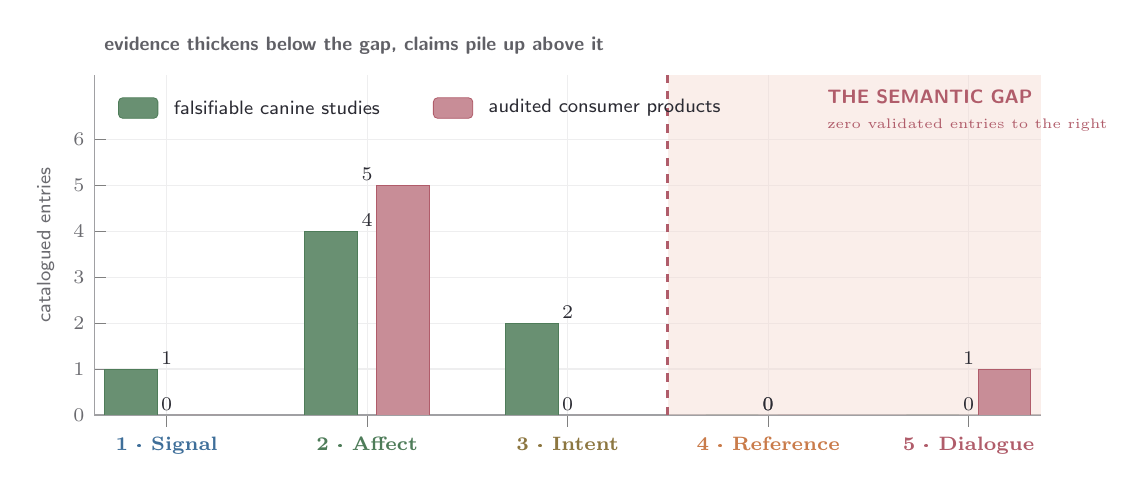
\begin{tikzpicture}[font=\sffamily]
  \begin{axis}[
      name=ev,
      width=13.6cm, height=5.9cm,
      ymin=0, ymax=7.4,
      symbolic x coords={1,2,3,4,5},
      xtick=data,
      xticklabels={%
        {\color{skydeep}\bfseries 1 \textperiodcentered\ Signal},
        {\color{sagedeep}\bfseries 2 \textperiodcentered\ Affect},
        {\color{gold!60!black}\bfseries 3 \textperiodcentered\ Intent},
        {\color{pawdeep}\bfseries 4 \textperiodcentered\ Reference},
        {\color{rosedeep}\bfseries 5 \textperiodcentered\ Dialogue}},
      ytick={0,1,2,3,4,5,6},
      tick label style={font=\scriptsize, text=ink!70},
      axis lines*=left, line width=0.6pt, draw=ink!45,
      ylabel near ticks, ylabel style={font=\sffamily\scriptsize, text=ink!70},
      ylabel={catalogued entries},
      grid=major, grid style={ink!8},
      ybar=7pt, bar width=19pt,
      every node near coord/.style={font=\sffamily\bfseries\scriptsize,
        text=ink, anchor=south, inner sep=1.5pt},
      enlarge x limits=0.09,
    ]
    % shaded region: above the gap, nothing has been validated
    \path (axis cs:3,0) -- (axis cs:4,0) coordinate[midway] (gapx);
    \fill[gap, opacity=0.45] (gapx |- current axis.south)
      rectangle (current axis.north east);
    \addplot+[ybar, mark=none, fill=sagedeep!85, draw=sagedeep, line width=0.3pt,
              nodes near coords]
      coordinates {(1,1) (2,4) (3,2) (4,0) (5,0)};
    \addplot+[ybar, mark=none, fill=rosedeep!70, draw=rosedeep, line width=0.3pt,
              nodes near coords]
      coordinates {(1,0) (2,5) (3,0) (4,0) (5,1)};
    \draw[dashed, rosedeep, line width=1.1pt] (gapx |- current axis.south)
      -- (gapx |- current axis.north);
  \end{axis}

  % hand-drawn legend: solid swatches in one row, clear of the bars
  \node[fill=sagedeep!85, draw=sagedeep, line width=0.3pt, rounded corners=1.5pt,
        minimum width=0.5cm, minimum height=0.26cm, inner sep=0, anchor=west] (sw1)
    at ($(ev.north west)+(0.30cm,-0.42cm)$) {};
  \node[font=\sffamily\scriptsize, text=ink, anchor=west] (l1)
    at (sw1.east) {\;falsifiable canine studies};
  \node[fill=rosedeep!70, draw=rosedeep, line width=0.3pt, rounded corners=1.5pt,
        minimum width=0.5cm, minimum height=0.26cm, inner sep=0, anchor=west] (sw2)
    at ($(l1.east)+(0.55cm,0)$) {};
  \node[font=\sffamily\scriptsize, text=ink, anchor=west] (l2)
    at (sw2.east) {\;audited consumer products};

  \node[font=\sffamily\bfseries\scriptsize, text=rosedeep, align=left,
        anchor=north west]
    at ($(gapx |- ev.north west)+(1.9cm,-2pt)$)
    {THE SEMANTIC GAP\\[1pt]{\sffamily\tiny\normalfont zero validated entries to the right}};
  \node[font=\sffamily\bfseries\scriptsize, text=ink!75, anchor=south west]
    at ($(ev.north west)+(0pt,4pt)$) {evidence thickens below the gap, claims pile up above it};
\end{tikzpicture}
}
\caption{Catalogued entries per rung of the ladder. Green: the canine studies
of Table~\ref{tab:evidence} that carry an independent error signal, assigned
to the rung each study reaches (the growl study spans rungs 2--3 and is
counted at rung 2; the bark-to-sentence row is excluded from this series).
Rose: the audited products of Table~\ref{tab:products} at their actual rung
(DogTok, a command-to-bark aid, has no receptive rung and is left out), plus
the bark-to-sentence category placed at the rung it claims. The shaded
region is the semantic gap of Figure~\ref{fig:ladder}: nothing to its right
has been validated.}
\label{fig:evidence}
\end{figure}

\begin{table}[htbp]
\centering
\caption{Consolidated limitations of canine ``translation,'' with locus and
consequence.}
\label{tab:limits}
\footnotesize
\setlength{\tabcolsep}{4pt}
\begin{tabular}{@{}p{4.0cm}p{4.6cm}p{5.0cm}@{}}
\toprule
\textbf{Limitation} & \textbf{Where it bites} & \textbf{Consequence} \\
\midrule
No ground-truth message & bark-to-sentence scoring & fidelity is unfalsifiable \\
Human-perceived labels & Rung-2 metrics & a proxy for state, not a readout \\
Undisclosed protocols & vendor accuracies & claims cannot be checked \\
Clever Hans / anthropomorphism & uncontrolled home use & the observer leaks the answer \\
No parallel corpus & supervised training & no translation signal exists \\
Semantic gap / no recursion & Rung 5 & the target may not exist \\
Fluency $\neq$ fidelity & LLM sentence rendering & hallucinated ``translations'' \\
No closed-loop error signal & consumer market & the field cannot self-correct \\
\bottomrule
\end{tabular}
\end{table}

\section{The Evaluation Crisis: Why the Numbers Cannot Be Trusted}
\label{sec:eval}

If the ladder tells us \emph{what} could be translated, the evaluation
problem tells us why we cannot yet know \emph{whether} it has been. This
section argues that the field's most quoted quantities---vendor accuracies
above 80\%, press-release superlatives---are, as presently defined,
\emph{unfalsifiable}, and that fixing this is a prerequisite for calling any
system a translator.

\subsection{The ground-truth problem}
Translation, in the human sense, is scored against a reference: a bilingual
corpus supplies the intended meaning, and metrics such as BLEU or human
adequacy judgments measure fidelity to it. Canine communication has no such
reference. There is no canonical ``intended message'' behind a bark, no
bilingual informant who can confirm that ``I want to play'' is what the dog
meant. The dog cannot report its intent, and---per
Section~\ref{sec:biology}---there may be no sentence-shaped intent to report.
Consequently, a bark-to-sentence system cannot be scored for translational
fidelity at all. What \emph{can} be scored is the upstream classifier: does
the model's emotion label agree with a human consensus label on a held-out
recording? That is a Rung-2 metric, and it is the only honest number in the
pipeline. Reporting it as a ``translation accuracy'' is a category mistake.

\subsection{What the vendor numbers actually are}
When a product advertises ``81.5\% accuracy,'' the defensible reading is:
on some internal test set, the predicted emotion class matched a
human-assigned class 81.5\% of the time. Three problems follow. First, the
test set, label protocol, class balance, and inter-annotator agreement are
rarely disclosed, so even the Rung-2 claim cannot be independently checked.
Second, the label is the \emph{human-perceived} emotion or the
\emph{eliciting context}, which is a proxy for the dog's state, not a
readout of it; the ELTE tradition is explicit about
this~\cite{pongracz2006acoustic,icassp2018dogbark}. Third, the rendered
sentence is produced \emph{after} classification by a language model
optimized for human resonance, so its fidelity is never measured at all.
The number thus travels down the pipeline as marketing while its meaning
stays fixed at the top.

\subsection{Unfalsifiability and the absent complaint}
A scientific claim must be falsifiable: there must be some observation that
could show it false. ``This bark means `I love you'\,'' admits no such
observation---the dog will not contradict it, and any subsequent behavior
can be retrofitted to the narrative. This is the structural reason the
consumer market cannot self-correct: there is no error signal. Compare a
weather forecast, which is scored against tomorrow's weather, or a
speech-to-text system, scored against a transcript. The pet translator has
no tomorrow and no transcript. Until a validation loop supplies an error
signal, its outputs are unfalsifiable interpretations, not measurements.

\subsection{Clever Hans, anthropomorphism, and the observer effect}
Two classic threats compound the problem. The \emph{Clever Hans} effect---%
the horse that appeared to do arithmetic but was reading its trainer's
unconscious cues---is the permanent hazard of any animal-communication
experiment: the human observer leaks the answer. Soundboard studies guard
against this with blind protocols and unfamiliar
button-pressers~\cite{bastos2024plos}; consumer apps, used by the devoted
owner in an uncontrolled home, do the opposite. \emph{Anthropomorphism} is
the second threat: attributing human propositional attitudes (``she says
she loves me'') to graded affective signals. The critical-review literature
on canine emotion perception warns that human observers project their own
categories onto the dog~\cite{sci2022explainable}, and a language model
trained on human text will amplify exactly this projection. The product
thus risks teaching owners to \emph{ignore} the dog's real body signals in
favor of a flattering sentence---a welfare harm we return to in
Section~\ref{sec:ethics}.

\subsection{What a valid evaluation would require}
A defensible evaluation program has four ingredients.
\begin{enumerate}[label=(\arabic*)]
  \item \textbf{Defined labels and disclosed protocols.} Report Rung-2
  metrics on a public, held-out corpus with inter-annotator agreement, class
  balance, and per-class confusion---the BEANS/BirdSet discipline applied to
  dogs~\cite{hagiwara2023beans}.
  \item \textbf{Calibration, not just accuracy.} Output probabilities that
  match observed frequencies, so a welfare tool can threshold responsibly.
  \item \textbf{Closed-loop validation.} Test inferred intent against the
  dog's subsequent behavior under blind conditions---the playback logic of
  Section~\ref{sec:pipeline}, adapted to the home.
  \item \textbf{Separate the sentence from the score.} Never report a
  generative rendering as evidence of fidelity; treat it as a user-interface
  layer, clearly labeled as interpretation.
\end{enumerate}
None of today's consumer products satisfies these. The research community
satisfies (1) and (2) in patches and (3) in the soundboard and cross-species
literature. The gap between the two is the evaluation crisis.

\subsection{A falsifiability criterion for the field}
We propose a simple demarcation: \emph{a canine communication system should
be called a translator only if its outputs are scored against an
independent, animal-grounded error signal.} By this criterion, no current
product qualifies; the soundboard paradigm qualifies at the word level;
and the rest is affect classification with a narrative interface. This is
not pedantry. It is the difference between a measurement and a story, and
the field's credibility---and the animals' welfare---depends on keeping them
apart.
\section{So How Far Are We? An Honest Distance Estimate}
\label{sec:distance}

We can now answer the title question without evasion. The answer is not a
number of years but a map: the distance depends entirely on which rung of
the ladder one means, and the rungs differ not by degree but by kind.
Table~\ref{tab:distance} gives our estimate, with the evidence and the
dominant blocker for each.

\subsection{Rung 1--2: essentially here, and useful}
Signal detection and affect classification are solved in the laboratory
and shipping in products. The remaining work is engineering and
validation---public benchmarks, calibration, multimodal fusion---not
discovery. A calibrated, validated welfare monitor that reports arousal and
valence with honest uncertainty is plausibly a \textbf{2--4 year} horizon
from the research frontier to reliable deployment. This is the genuinely
useful payoff: early stress or pain detection, shelter welfare assessment,
veterinary triage. It is not ``translation,'' and calling it such would
oversell it; but it is real.

\subsection{Rung 3: a foothold, a decade of work}
Intent and context inference on \emph{natural} signals is emerging. The
soundboard literature proves that referential intent exists and is
checkable~\cite{bastos2024plos,bastos2024scirep}, but it does so with
human-supplied symbols. Extending this to spontaneous barks, faces, and
postures---fusing modalities, modeling goals, validating closed-loop---is a
research program, not a product cycle. We estimate \textbf{validated
natural-signal intent inference at roughly 2030 or later}, contingent on
the evaluation infrastructure of Section~\ref{sec:eval} being built. The
blocker is not model capacity; it is labeled, grounded, validated data.

\subsection{Rung 4--5: possibly never, and that is informative}
Open referential translation and free dialogue presuppose a generative
symbolic system in the dog that the biological evidence does not support.
Here the honest answer is \textbf{no credible timeline}, and the reason is
not pessimism about AI but a fact about the subject: there may be no
language there to translate. This is the survey's central, deflationary
claim. It does not rule out an \emph{engineered} dialogue---structured
human-to-dog input via trained symbols, with the dog responding through a
soundboard---which is a Rung-3 artifact wearing Rung-5 clothing. But faithful
translation of spontaneous canine ``speech'' into English sentences is, in
the strong sense, possibly ill-posed, and more compute will not fix a
category error.

\subsection{Why ``more scale'' is not the answer}
It is tempting to read the cross-species successes as evidence that scaling
foundation models will eventually crack the dog. The reading is mistaken.
CETI, DolphinGemma, and the finch models advance \emph{structure discovery
and generation}---the front of the pipeline. They do not supply semantics,
and their authors say so~\cite{sharma2024whale,google2025dolphingemma}. The
canine bottleneck is at the \emph{back} of the pipeline (grounding,
validation) and, above Rung 3, in the subject itself. Scaling the encoder
makes Rung 1--2 better; it does not create a grammar that is not there.
The distance to Rung 5 is therefore not a function of parameters but of
biology.

\subsection{The reframe: from translation to interpretation}
The productive move is to stop asking ``when will we translate dogs?'' and
start asking ``how well can we \emph{interpret} canine state, with calibrated
uncertainty and animal-grounded validation?'' That question has answers,
has metrics, and has welfare value. It also respects the animal: it treats
the dog as a signaler with its own modalities, not as a defective human
whose sentences we are waiting to recover. The Rosetta Stone that titles
this survey is, in the end, a warning as much as a promise: there may be no
decree to transcribe (Section~\ref{sec:conclusion}).

\begin{table}[htbp]
\centering
\caption{Distance estimate by rung. Horizons are judgments from the
evidence reviewed, not predictions; ``blocker'' names the dominant
obstacle. Rungs 4--5 are marked possibly ill-posed because the requisite
generative symbolic system is not evidenced in natural canine communication.}
\label{tab:distance}
\small
\begin{tabular}{@{}p{2.7cm}p{2.5cm}p{4.0cm}p{3.6cm}@{}}
\toprule
\textbf{Rung} & \textbf{Status} & \textbf{Horizon} & \textbf{Dominant blocker} \\
\midrule
1 Signal & Solved & Now & Engineering only \\
2 Affect & Shipping & 2--4 yr to validated welfare use &
Calibration, public benchmarks \\
3 Intent & Foothold & $\sim$2030+ & Grounded, validated data \\
4 Reference & Unproven & No credible timeline & No productive symbol system \\
5 Dialogue & Possibly ill-posed & Possibly never & No evidenced generative grammar \\
\bottomrule
\end{tabular}
\end{table}
\section{Ethics: The Animal as Partner}
\label{sec:ethics}

A technology that claims to read an animal's mind carries obligations an
ordinary classifier does not. The most immediate is welfare: an owner told
``she says she loves you'' may overlook the flattened ears, the whale eye,
the lip lick that signal stress, and an owner told ``my tummy hurts'' may
over-react or dismiss genuine pain when the app stays silent. Human
observers already project their categories onto dogs, reading a
stress-driven appeasement face as guilt~\cite{sci2022explainable,horowitz2009disambiguate},
and a resonant language model amplifies the projection. Welfare-first design therefore surfaces calibrated state
estimates with uncertainty rather than sentences, never overrides
observable body signals, routes high-stakes inferences (pain, aggression,
distress) to human or veterinary review, and collects passively, without
induced stress to elicit training barks.

Honesty follows from the evaluation crisis: separate the calibrated
classifier from the narrative interface, label the latter as
interpretation, disclose that accuracy figures refer to emotion
classification, and refrain from unvalidated reverse-direction claims.
Privacy follows from the always-on home sensor: on-device inference where
possible (the DolphinGemma-on-Pixel precedent is
instructive~\cite{google2025dolphingemma}), minimal retention, explicit
household consent for cloud training, and clear deletion. The animal cannot
consent; the household must, and the design should make that consent
meaningful.

Finally, a conceptual obligation. Treating the dog as an oracle whose
``words'' we extract flattens its communicative life into a human format.
The soundboard paradigm is ethically attractive precisely because it treats
the dog as a partner in a negotiated symbol system, with the dog's behavior
as the check~\cite{bastos2024plos,bastos2024scirep}; CETI's leadership has
likewise stressed that breakthroughs in whale communication should be a
collective human decision, with responsible-interaction guidelines before
signals are sent to wild animals. This framework inherits the consensus
principles of responsible AI (transparency, justice, non-maleficence,
responsibility, privacy)~\cite{jobin2019global}, the documented gap between
principles and practice~\cite{mittelstadt2019principles,floridi2018ai4people},
the political-economy critique of hidden data and labor supply
chains~\cite{crawford2021atlas}, the risk-tiered regulatory baseline of
the EU AI Act~\cite{european2024aiact}, and the concrete engineering of
fair, safe, and human-compatible systems---disparate-impact auditing,
specification-gaming avoidance, and compatibility~\cite{barocas2016bigdata,amodei2016concrete,russell2019human}. On the animal side, the precautionary
principle for sentience warrants moral consideration under
uncertainty~\cite{birch2017precaution}, and recent work locates the edge of
sentience in exactly the graded affective capacities this survey treats as
decodable~\cite{birch2024edge}. The synthesis is a double obligation: be
honest about what the model knows, and be careful toward what the animal
feels.

For builders and reviewers, the framework condenses to six checks: report
Rung-2 metrics on public held-out data with calibration, never as
``translation accuracy''; separate and label interpretation versus
measurement; validate intent claims closed-loop and blind or call them
hypotheses; collect passively, infer on-device, minimize retention, obtain
meaningful consent; route high-stakes outputs to human or veterinary review
and never override body signals; and treat the animal as a partner, keeping
welfare as the terminal criterion. None of this slows the useful science;
all of it protects the animals and the credibility of the field.

\section{A Research Agenda: What Would Actually Move the Needle}
\label{sec:future}

If the distance estimate of Section~\ref{sec:distance} is right, then the
highest-leverage work is not bigger models but better \emph{infrastructure
and protocols}. We propose a concrete agenda, ordered by leverage.

\subsection{A public, grounded canine corpus}
The field lacks what BEANS and BirdSet provide for general bioacoustics: a
standardized, public, multimodal canine corpus with agreed
labels~\cite{hagiwara2023beans}. The ideal corpus pairs synchronized audio,
video (DogFACS-codeable face and posture), context metadata, and---crucially%
---\emph{consequent behavior}, so that intent hypotheses can be checked. The
soundboard citizen-science network, with thousands of instrumented homes,
is the natural collection substrate~\cite{bastos2024plos}. Building this
corpus with disclosed protocols and inter-annotator agreement would do more
for the field than any single model release.

\subsection{Calibrated, multimodal affect models}
On the modeling side, the priority is fusion and calibration: combine bark,
growl, face, and posture into a single state estimate with honest
uncertainty, trained and evaluated on the public corpus. Self-supervised
encoders (AVES, NatureLM-audio, Perch) supply the
backbone~\cite{hagiwara2023aves,robinson2024naturelm,ghani2023perch}; the
contribution is the canine-specific grounding and the calibration layer
that makes the output safe for welfare use.

\subsection{Closed-loop intent validation}
The methodological frontier is the validation loop: infer an intent, act on
it (or emit a candidate signal), and test the dog's response under blind
conditions. The soundboard and CHAT protocols are the
templates~\cite{bastos2024scirep,google2025dolphingemma}. A home-adapted,
owner-blind protocol that scores intent inference against the dog's
subsequent behavior would supply the error signal the field lacks
(Section~\ref{sec:eval}) and turn Rung 3 from hypothesis into measurement.

\subsection{Structure discovery, with humility}
Applying sequence-structure methods to bark corpora is worth doing---but
with the explicit prior that canine displays are graded and may yield no
clean combinatorial alphabet. The CETI and DolphinGemma toolkits are
available~\cite{sharma2024whale,google2025dolphingemma}; the discipline is to
report structure as form, not meaning, and to heed the acoustic-similarity
critique~\cite{yovel2025critique}. A negative result---no discrete
inventory---would itself be valuable, sharpening the semantic-gap claim.

\subsection{Engineered dialogue, not extracted dialogue}
The most promising path to anything resembling conversation is
\emph{engineered}: expand the soundboard paradigm into a richer, negotiated
symbol system, with the dog as partner and the behavior as check. This is
Rung-3 work that may eventually look like dialogue, without pretending that
spontaneous barks contain sentences. It is also the ethically preferable
path (Section~\ref{sec:ethics}).

\subsection{What would falsify our thesis}
A good survey states what would change its mind. Our central claim---that
Rungs 4--5 are ill-posed for natural canine communication---would be
undermined by: (i) a reproducible demonstration of a productive, open
referential vocabulary in spontaneous dog signals, validated by playback;
or (ii) evidence of recursive, generative combination in natural canine
displays (not trained soundboard sequences). Absent such evidence, the
ladder stands. We invite the community to try to falsify it; that is how
the distance estimate should shrink.
\section{Conclusion}
\label{sec:conclusion}

We began with a folkloric question---how far are we from translating what a
dog says?---and end with a deflationary but, we hope, more useful answer.
``Translation'' is not one capability but five, and the distance to each is
different in kind, not merely in degree. Signal detection and affect
classification (Rungs 1--2) are here and shipping; validated affect-and-intent
inference (Rung 3) is a research program with a foothold in the soundboard
literature and a plausible horizon around 2030; open referential translation
and free dialogue (Rungs 4--5) presuppose a generative symbolic system that
the biological evidence does not support, and may be permanently ill-posed.
The canine Rosetta Stone is, in the end, a metaphor with a catch: the
original worked because one decree existed in three scripts, and for the
dog there may be no decree to transcribe---only a rich, graded, affective
life we can learn to read but not to render as sentences.

Three findings anchor this verdict. First, the biology: dogs signal affect,
arousal, identity, motivation, and---with human scaffolding---referential
intent, but they do not possess an open-ended generative
grammar~\cite{pongracz2005barks,farago2017growls,waller2013dogfacs,bastos2024scirep}.
Second, the technology: the decoding pipeline's front (encoding, structure
discovery) is maturing fast on the back of the cross-species foundation-model
boom, while its back (grounding, validation) is where canine-specific work
is needed and where commercial effort is
absent~\cite{hagiwara2023aves,robinson2024naturelm,sharma2024whale,google2025dolphingemma}.
Third, the evaluation: the field's headline accuracies are unfalsifiable as
translation metrics, because no ground-truth intended message exists to
score against; they are, at best, Rung-2 emotion-classification
numbers~\cite{icassp2018dogbark}. The commercial market demonstrates Rung 2
and sells Rung 5, and the gap between those is the subject of this survey.

The way forward is not more scale but better infrastructure and protocols:
a public grounded canine corpus, calibrated multimodal affect models,
closed-loop blind validation, and an ethics framework that treats the animal
as a partner and keeps welfare as the terminal criterion. The useful,
achievable goal is \emph{interpretation with calibrated uncertainty}, not
transcription of a language that may not exist. That goal is within reach
this decade, and it is worth reaching.

\subsection{Limitations of this survey}
In the spirit of evidence-bounded research, we state the limitations
plainly. (1)~This is a narrative survey, not a PRISMA systematic review;
sources were gathered through structured web and literature search in
November 2026, and coverage is broad rather than exhaustive. (2)~Several
fast-moving items (WhAM, ZF-AIM, vendor metrics) rest on project reports and
journalism rather than peer review, and are labeled as such; commercial
accuracies are reported \emph{as claims} and were not independently
verified. (3)~Some citations were confirmed to the level of venue, year,
and DOI via secondary indexes rather than full-text retrieval; a
production version should verify each against the primary record.
(4)~The distance estimates are expert judgments from the reviewed evidence,
not forecasts, and Section~\ref{sec:future} states what would falsify them.
These limitations do not weaken the central claim---they bound it, which is
the point.

\subsection*{Acknowledgments and tools}
This survey was prepared with the assistance of open research-agent
tooling, including the Scientific Agent Skills literature-review and
autoresearch workflows~\cite{kassis2026skills}, which contributed the
search-documentation and citation-verification discipline used here. The
figures are original TikZ constructions released with the repository for
reuse and correction.

\subsection*{Data and code availability}
The \LaTeX\ source, both hero figures, the bibliography, and the project
page are openly available in the \texttt{woof-to-word} repository:
\url{https://github.com/mcxiaoxiao/woof2word}. Corrections and
falsification attempts are welcome.

\section*{References}
\addcontentsline{toc}{section}{References}
\begin{thebibliography}{99}
\small

\bibitem{pongracz2005barks}
P.~Pongr\'acz, C.~Moln\'ar, A.~Mikl\'osi, and V.~Cs\'anyi,
``Human listeners are able to classify dog (\emph{Canis familiaris}) barks
recorded in different situations,''
\emph{Journal of Comparative Psychology}, vol.~119, no.~2, pp.~136--144, 2005.

\bibitem{pongracz2006acoustic}
P.~Pongr\'acz, C.~Moln\'ar, and A.~Mikl\'osi,
``Acoustic parameters of dog barks carry emotional information for humans,''
\emph{Applied Animal Behaviour Science}, vol.~100, no.~3--4, pp.~228--240, 2006.

\bibitem{molnar2006discriminate}
C.~Moln\'ar, P.~Pongr\'acz, A.~D\'oka, and A.~Mikl\'osi,
``Can humans discriminate between dogs on the basis of the acoustic parameters
of barks?'' \emph{Behavioural Processes}, vol.~73, no.~1, pp.~76--83, 2006.

\bibitem{farago2017growls}
T.~Farag\'o, N.~Tak\'acs, A.~Mikl\'osi, and P.~Pongr\'acz,
``Dog growls express various contextual and affective content for human
listeners,'' \emph{Royal Society Open Science}, vol.~4, p.~170134, 2017.

\bibitem{icassp2018dogbark}
``What is my dog trying to tell me? The automatic recognition of the context
and perceived emotion of dog barks,'' in \emph{Proc.\ IEEE ICASSP}, 2018.
DOI: 10.1109/ICASSP.2018.8461757.

\bibitem{waller2013dogfacs}
B.~M. Waller, K.~Peirce, C.~C. Caeiro, et~al.,
``DogFACS: The dog facial action coding system,'' 2013.
Available: \url{https://www.animalfacs.com}.

\bibitem{kaminski2017attention}
J.~Kaminski, J.~Waller, R.~Diogo, A.~Hartstone-Rose, and A.~M. Burrows,
``Human attention affects facial expressions in domestic dogs,''
\emph{Scientific Reports}, vol.~7, p.~13066, 2017.

\bibitem{sci2024domestication}
``Domestication constrains the ability of dogs to convey emotions via facial
expressions in comparison to their wolf ancestors,''
\emph{Scientific Reports}, 2024. DOI: 10.1038/s41598-024-61110-6.

\bibitem{sci2022explainable}
``Explainable automated recognition of emotional states from canine facial
expressions,'' \emph{Scientific Reports}, 2022.
DOI: 10.1038/s41598-022-27079-w.

\bibitem{sci2023cnnewoa}
``Pet dog facial expression recognition based on convolutional neural network
and improved whale optimization algorithm,'' \emph{Scientific Reports}, 2023.
DOI: 10.1038/s41598-023-30442-0.

\bibitem{sci2025automated}
``Automated analysis of emotional expressions in dogs,''
\emph{Scientific Reports}, 2025. DOI: 10.1038/s41598-025-15741-y.

\bibitem{sci2025landmarks}
``Dog facial landmarks detection and its applications for facial analysis,''
\emph{Scientific Reports}, 2025. DOI: 10.1038/s41598-025-07040-3.

\bibitem{kaminski2004rico}
J.~Kaminski, J.~Call, and J.~Fischer,
``Word learning in a domestic dog: Evidence for ``fast mapping'',''
\emph{Science}, vol.~304, no.~5677, pp.~1682--1683, 2004.

\bibitem{pilley2011chaser}
J.~W. Pilley and A.~K. Reid,
``Border collie comprehends object names as verbal referents,''
\emph{Behavioural Processes}, vol.~86, no.~2, pp.~184--195, 2011.

\bibitem{bastos2024plos}
A.~P.~M. Bastos, A.~Evenson, P.~M. Wood, et~al.,
``How do soundboard-trained dogs respond to human button presses? An
investigation into word comprehension,'' \emph{PLoS ONE}, vol.~19,
p.~e0307189, 2024. DOI: 10.1371/journal.pone.0307189.

\bibitem{bastos2024scirep}
A.~P.~M. Bastos, Z.~N. Houghton, L.~Naranjo, and F.~Rossano,
``Soundboard-trained dogs produce non-accidental, non-random and non-imitative
two-button combinations,'' \emph{Scientific Reports}, vol.~14, p.~28771, 2024.
DOI: 10.1038/s41598-024-79517-6.

\bibitem{animalcog2025review}
``Let's talk about ``talking'' dogs! Reviewing the science of soundboard
use,'' \emph{Animal Cognition}, 2025. PMC12367964.

\bibitem{bastos2023interact}
A.~P.~M. Bastos and F.~Rossano,
``Soundboard-using pets?'' \emph{Interaction Studies}, vol.~24, no.~2,
pp.~311--334, 2023. DOI: 10.1075/is.22050.pin.

\bibitem{sharma2024whale}
P.~Sharma, S.~Gero, R.~Payne, D.~F. Gruber, D.~Rus, A.~Torralba, and J.~Andreas,
``Contextual and combinatorial structure in sperm whale vocalisations,''
\emph{Nature Communications}, vol.~15, p.~3617, 2024.
DOI: 10.1038/s41467-024-47221-8.

\bibitem{andreas2022ceti}
J.~Andreas, G.~Begu\v{s}, M.~M. Bronstein, et~al.,
``Toward understanding the communication in sperm whales,''
\emph{iScience}, vol.~25, p.~104393, 2022.

\bibitem{google2025dolphingemma}
Google DeepMind, Georgia Tech, and Wild Dolphin Project,
``DolphinGemma: How Google AI is helping decode dolphin communication,''
Project report, 14 April 2025.

\bibitem{wham2025}
Project CETI, ``WhAM: Whale Acoustics Model,'' Technical report, 2025.

\bibitem{arxiv2025whaletrans}
``Towards a translative model of sperm whale vocalization,''
\emph{arXiv:2512.02206}, 2025.

\bibitem{hagiwara2023aves}
M.~Hagiwara, ``AVES: Animal vocalization encoder based on self-supervision,''
in \emph{Proc.\ IEEE ICASSP}, 2023.

\bibitem{robinson2024naturelm}
D.~Robinson, M.~Miron, M.~Hagiwara, and O.~Pietquin,
``NatureLM-audio: An audio--language foundation model for bioacoustics,''
\emph{arXiv:2411.07186}, 2024.

\bibitem{ghani2023perch}
B.~Ghani, T.~Denton, S.~Kahl, and H.~Klinck,
``Global birdsong embeddings enable superior transfer learning for bioacoustic
classification,'' \emph{Scientific Reports}, vol.~13, p.~22876, 2023.

\bibitem{hagiwara2023beans}
M.~Hagiwara et~al., ``BEANS: The benchmark of animal sounds,''
in \emph{Proc.\ IEEE ICASSP}, 2023.

\bibitem{openbeats2025}
``OpenBEATs: A fully open-source general-purpose audio encoder,''
\emph{arXiv:2507.14129}, 2025.

\bibitem{esp2026finch}
Earth Species Project and McGill University,
``ZF-AIM: An interactive zebra-finch vocalization model,'' Technical report,
2026 (not yet peer reviewed).

\bibitem{yovel2025critique}
Y.~Yovel, Commentary on acoustic-similarity pitfalls in animal-language
models, reported in \emph{Nature} news coverage, 2025--2026.

\bibitem{traini2024}
Traini (PetGPT / PEBI model), Commercial pet-empathy AI, 2024--2026.
Vendor-reported metrics; see Section~\ref{sec:products}.

\bibitem{bowlingual2002}
Takara Co., ``Bow-Lingual'' dog-bark translator, 2002.
Ig Nobel Peace Prize, 2002.

\bibitem{meowtalk2020}
J.~Sanchez (Akvelon), ``MeowTalk'' cat-vocalization app, 2020.

\bibitem{mengxiaoyi2026}
``Meng Xiao Yi'' pet translator (Alibaba Qwen-based; vendor-claimed 94.6\%),
2026. Reported via Chinese technology press.

\bibitem{petpuls2021}
Petpuls AI collar (Seoul National University spin-off), 2021.

\bibitem{quaranta2007tail}
A.~Quaranta, M.~Siniscalchi, and G.~Vallortigara,
``Asymmetric tail-wagging responses by dogs to different emotive stimuli,''
\emph{Current Biology}, vol.~17, no.~6, pp.~R199--R201, 2007.

\bibitem{andics2014voice}
A.~Andics, A.~G\'acsi, T.~Farag\'o, A.~Kis, and A.~Mikl\'osi,
``Voice-sensitive regions in the dog and human brain are revealed by
comparative fMRI,'' \emph{Current Biology}, vol.~24, no.~5, pp.~574--578, 2014.

\bibitem{kassis2026skills}
T.~Kassis, V.~Agarwal, Y.~He, D.~Patel, and A.~M. Brueckner,
``Scientific Agent Skills: A library of procedural knowledge for research
agents,'' \emph{arXiv:2609.00065}, 2026.
DOI: 10.48550/arXiv.2609.00065.

\end{thebibliography}

\end{document}